\documentclass[5p,authoryear]{elsarticle}
\makeatletter 
\def\ps@pprintTitle{%
 \let\@oddhead\@empty
 \let\@evenhead\@empty
 \let\@evenfoot\@oddfoot} % Supprimer le bas de page ELSEVIER
\makeatother
\usepackage[utf8]{inputenc} % En unicode
\usepackage[T1]{fontenc}
\usepackage[english]{babel}
\usepackage[babel=true]{csquotes} % permet de faire \enquote{a} (« a »)
\usepackage[fleqn]{amsmath} % pour certains signes mathématiques
\usepackage{amsthm} % Pour \begin{gather}
\usepackage{booktabs} % pour \toprule (un style de tableau)
\usepackage{multirow} % Pour colonnes multiples des tableaux
\usepackage{amssymb} % Pour \leqslant (<=, >=)
\usepackage{float}
\usepackage{hyperref} % 
\usepackage[english]{cleveref} 




%\bibliographystyle{elsarticle-num}
\bibliographystyle{elsarticle-harv}

\usepackage{fancyhdr}
\pagestyle{fancy}
\lhead{MSDS 458 - SEC 56}
\rhead{Lee, J.}

\begin{document}


\begin{frontmatter}

\title{Gambling Twitter Bot: \\Generative Recurrent Neural Networks}
\author{Jason Lee}
\address{Northwestern University, SPS \\Artificial Intelligence and Deep Learning \\2019FA MSDS 458-56}


\begin{abstract}

Generating original and coherent text with a machine is an incredibly difficult natural language processing (NLP) challenge. Typical machine learning algorithms are unable to accomplish this task. Language has many complicated patterns and subtle nuances that deep neural networks are able to detect. The goal of this study is to use generative recurrent neural networks (RNNs) to build chatbots that are able to compose original tweets in the voice of four distinct, high-profile twitter users in the sports betting community. The chatbots will be trained only on the specific user’s tweets and will have the ability to generate unprompted original tweets to share with the world.

\end{abstract}



\begin{keyword}
Generative Neural Networks (GNNs) \sep Recurrent Neural Networks (RNNs) \sep Deep Learning \sep Keras\end{keyword}

\end{frontmatter}



%\linenumbers
\section{Introduction}\label{introduction}

Typical machine learning algorithms are designed to create a basic output, either segmenting, classifying, or providing a predicted value based on the input data. However, with the many advances made in deep learning with powerful neural networks, algorithms are able to generate images, videos, songs, and sentences that are indistinguishable from their human made counterparts. These models are known as generative neural networks (GNNs) or generative adversarial networks (GANs) \citep{chollet}. Because of these great advances there are several new techniques in deep learning that provide a solid framework for data scientists to build “thinking” and “creative” artificial intelligence \citep{foster}. 

One of these new generative techniques, called variational autoencoders, can be used to completely change the facial expressions of people in photographs  \citep{VAEs}.Family pictures now, by way of variational encoders, have an easy way to get the parents, kids, and babies all smiling at the same time in a realistic way. Figure \ref{smile} shows an example of the progression an image goes through as the algorithm changes the facial expression from resting to smiling, moving from the original input image on the left to the final output on the right. 

\begin{figure}[!htb] \centering
	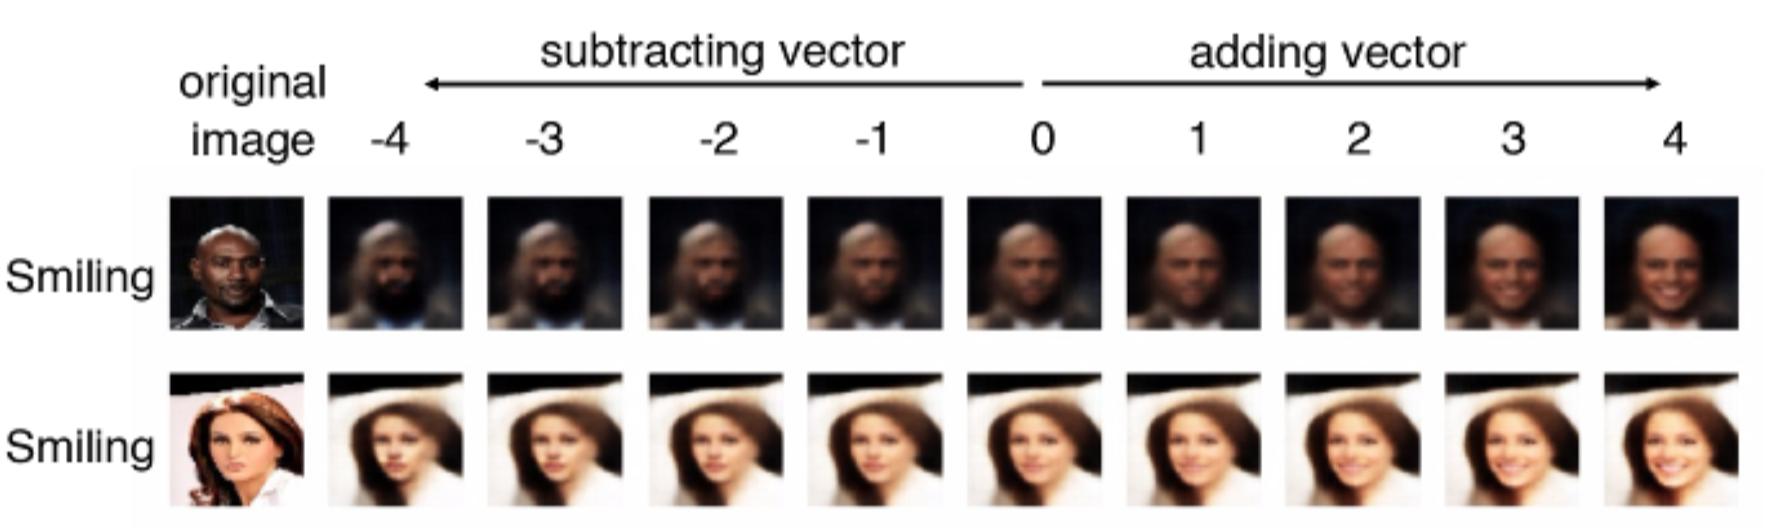
\includegraphics[width=3.4in]{figures/Smile_GAN.png}
	\caption[]{Deep neural network using variational autoencoders to change facial expressions in photos. The two original photos are on the left and as vectors are added or subtracted to the photo the expression changes} \label{smile} 
\end{figure}

Another new generative deep neural network, known as MuseGAN, was taught how to produce beautiful, new musical arrangements. The algorithm was built in such a way that it is able to create, without any input from a human, four bars of original music for an arrangement with bass, drums, guitar, piano, and strings \citep{MuseGAN}. Another MuseGAN was trained to help an artist create new songs. If the model is given one track, it will be able to generate four brand new accompanying tracks in the same style as the input track \citep{MuseGAN}.

There are other new generative algorithms in deep learning called CycleGANs that can be used to transfer specific styles across images \citep{CycleGAN}. 


\begin{figure}[!htb] \centering
	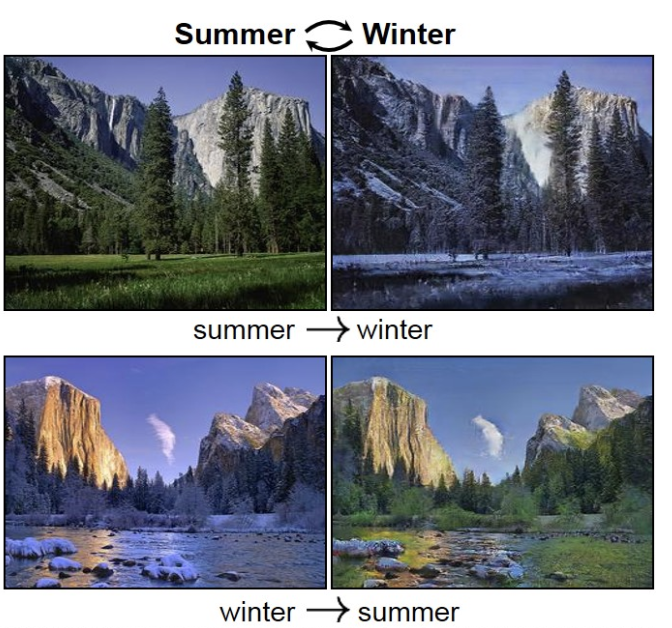
\includegraphics[width=3.4in]{figures/CycleGAN1.png}
	\caption[]{CycleGAN showing a change of style cycling between summer and winter with 2 landscape photographs} \label{summer} 
\end{figure}


\begin{figure}[!htb] \centering
	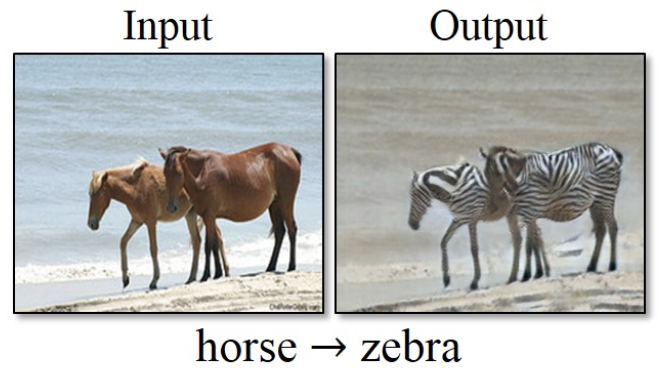
\includegraphics[width=3.4in]{figures/CycleGAN4.png}
	\caption[]{CycleGAN changing the style of a photograph with two horses on the beach to two zebras on the beach} \label{zebra} 
\end{figure}


\begin{figure}[!htb] \centering
	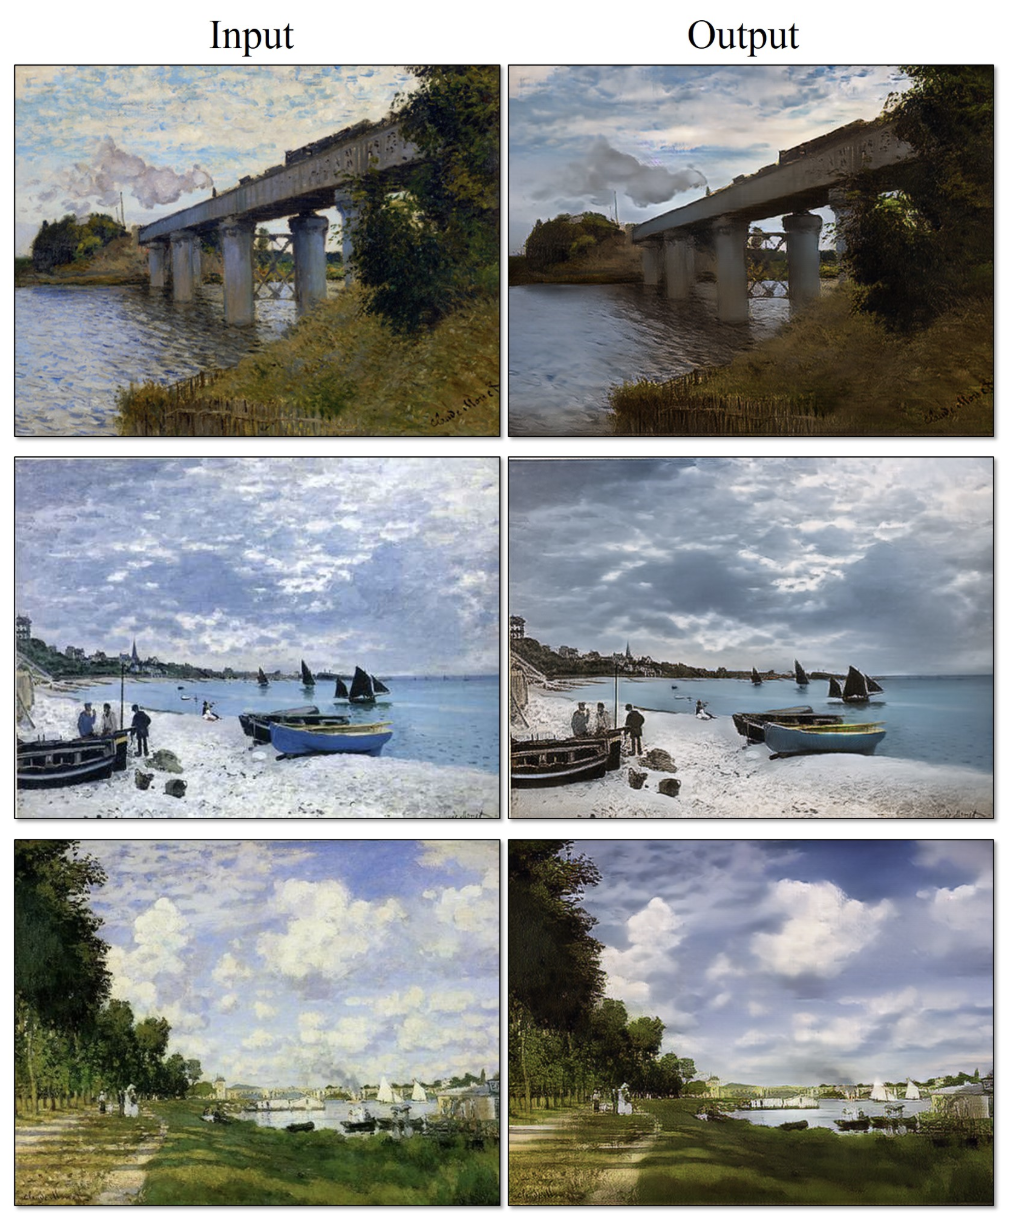
\includegraphics[width=3.4in]{figures/CycleGAN2.png}
	\caption[]{CycleGAN changing the style of three Monet paintings into realistic photographs} \label{monet} 
\end{figure}


\begin{figure}[!htb] \centering
	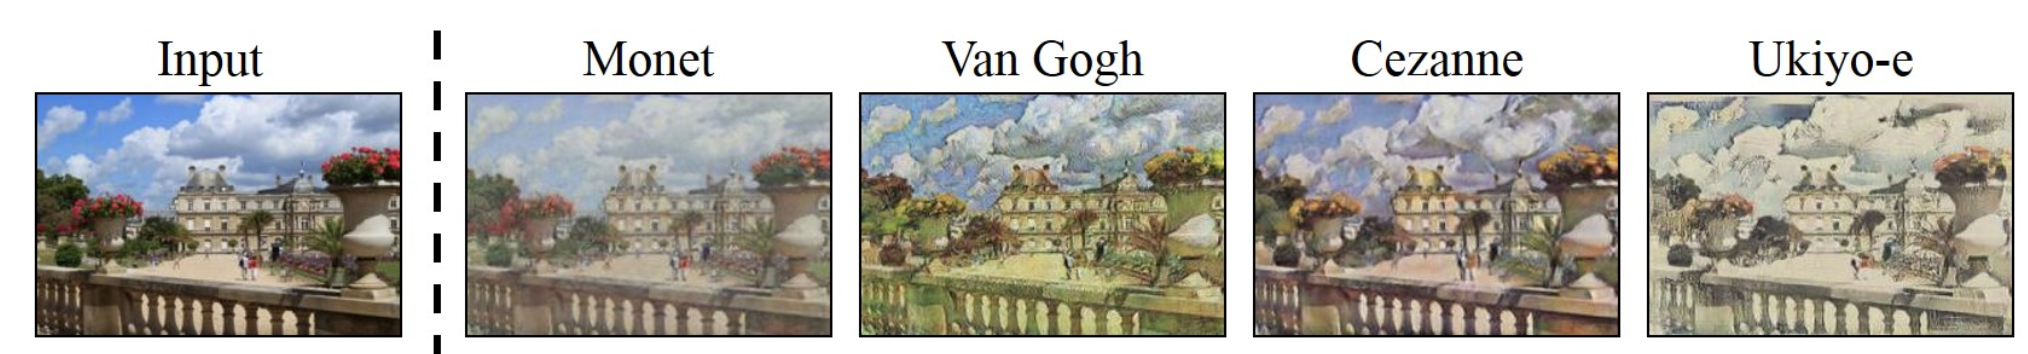
\includegraphics[width=3.4in]{figures/CycleGAN3.png}
	\caption[]{CycleGAN changing the style of a photograph into a painting in the distinctive styles of Monet, Van Gogh, Cezanne, and Ukiyo-e.} \label{paint} 
\end{figure}


Looking at figures \ref{summer}-\ref{paint}, the powerful work of the CycleGAN is shown. An image is changed from summer to winter and from winter to summer. Another image has horses that are seamlessly changed to zebras on the shore. Works from Monet fed through the CycleGAN are changed into natural photographs. Finally, a photograph is changed into the style of several distinct artists. It is incredibly difficult to discern the real pictures from the computer-generated pictures. These GANs are impressive enough to fool even the most astute observer. Figure \ref{wife} is a photograph fed into Google’s DeepDream algorithm and changed into new works of art. 

\begin{figure}[!htb] \centering
	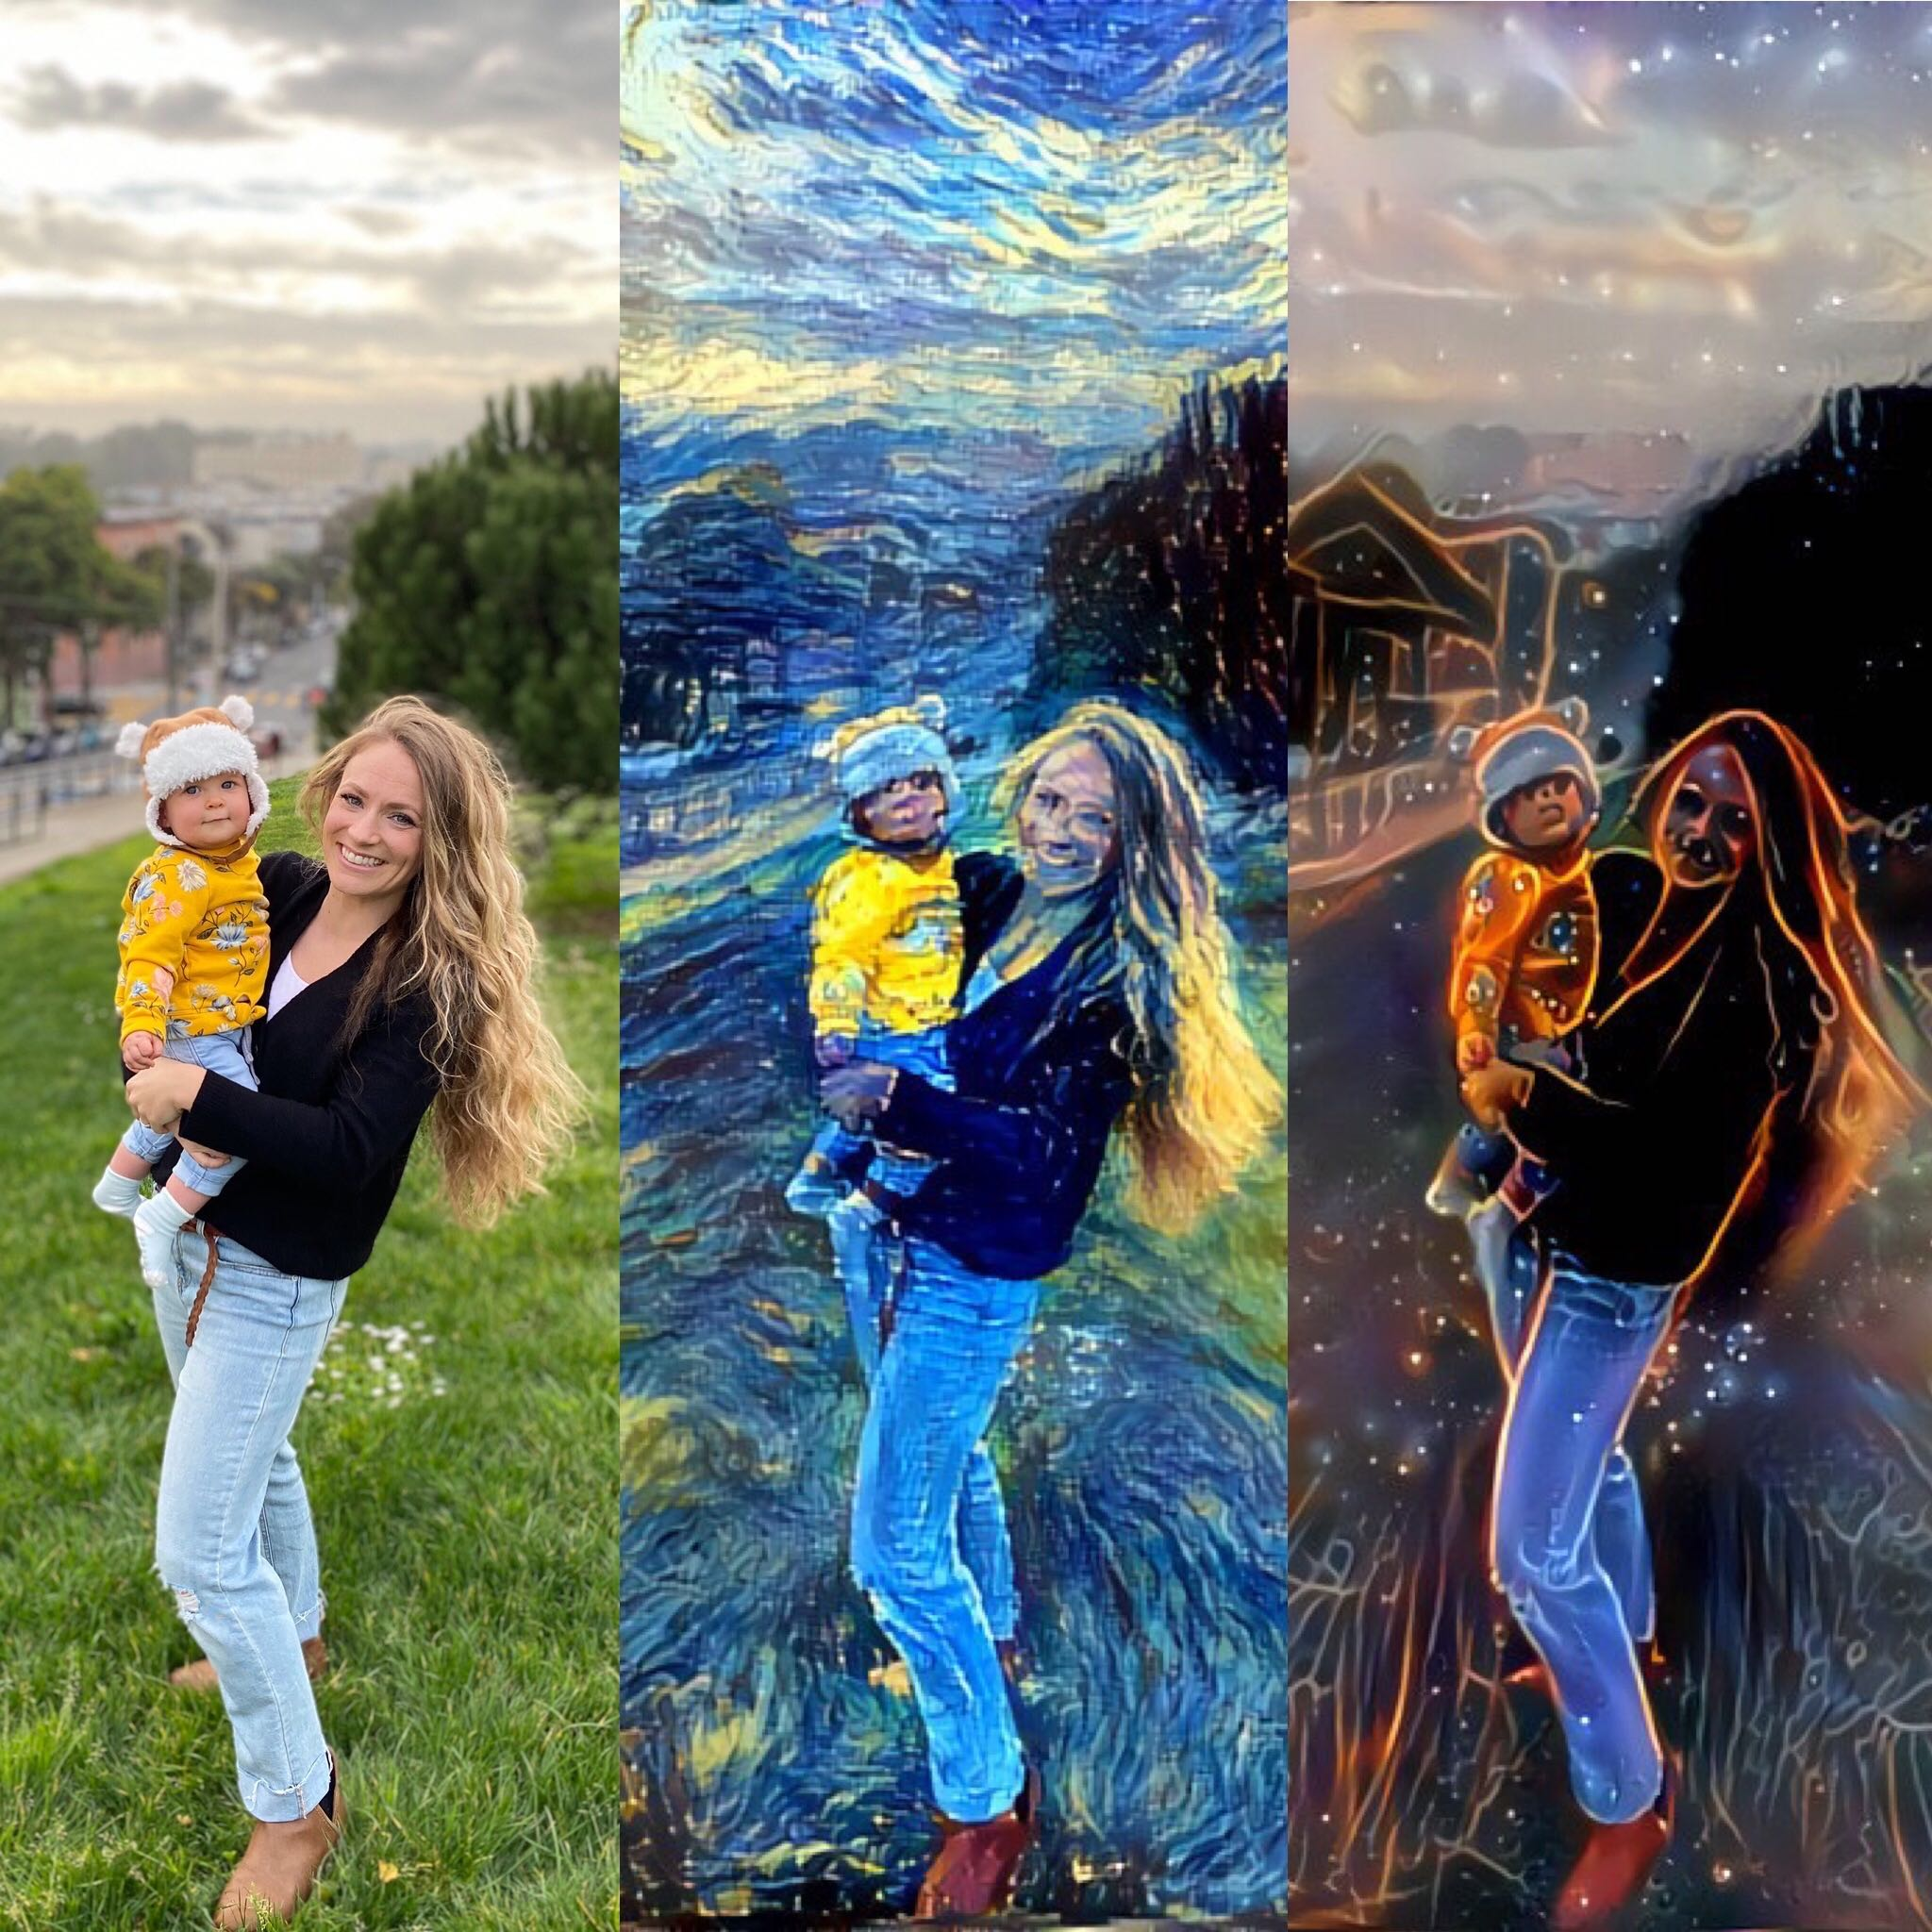
\includegraphics[width=3.4in]{figures/Perfection-DeepDream.jpg}
	\caption[]{DeepDream generated images from a photo of my beautiful wife and baby in San Francisco.} \label{wife} 
\end{figure}

Then there are generative recurrent neural networks that can be built to write new books, poems, or movie scripts. The entire script for the 2016 short film “Sunspring” was written by a recurrent neural network (RNN) algorithm with long short-term memory (LSTM) named Benjamin. The algorithm was trained on a corpus of 1980s and 1990s science fiction movie scripts \citep{movie}. Another recurrent neural network was trained on Eminem lyrics and used to write a new rap song \citep{slim}. 

These and many other generative deep learning models learn how to create new works of art. They are the type of models that spring into people’s minds when “Artificial Intelligence” is mentioned. 

This study focuses on using a generative recurrent neural network to build chatbots that are able to compose original tweets in the voice of four distinct, high-profile twitter users in the sports betting community. 

This project builds on the work completed in the previous natural language processing study classifying various Twitter users based on their tweets \citep{lee}. Instead of using the model to solve a classification problem, this project takes a step deeper into the artificial intelligence space. The new goal will be to build chatbots that can generate new tweets with the same subtly unique linguistic patterns as the gambling Twitter users they learn from. 

There are three specific desired outcomes for this project: 1 – Create working chatbots that are able to generate original content. 2 – Discover ways to improve the realism of the chatbots. 3 – Create a reproducible Python code workflow with functioning chatbot models to easily share with colleagues. 



\subsection{Popular Gambling Twitter Users} \label{twitter}

To accomplish the goal of this study, four popular twitter users in the sports betting community were selected who have distinctive tweeting styles. 


\begin{enumerate}
 \item Joseph Buchdahl (@12Xpert) – An academic, typically skeptical personality. Author of Squares and Sharps, Suckers and Sharks. 12.3k followers – 19.1k tweets.
 \item Joey Knish (@JoeyKnish22) – Everyday man from Detroit, Michigan. Quite possibly a degenerate gambler. 9.2k followers – 22.7k tweets.
 \item Micheal Schwimer (@mschwimer) – Former baseball player turned sports betting tout who was universally destroyed by the online sports betting community because of his “Trumpian” style touting service. 10.1k followers – 3.3k tweets.
 \item Pikachu Bets (@PikachuBets) – Angry sports bettor with a weird obsession with Pokemon. Takes pleasure in exposing frauds in the sports betting community like Michael Schwimer, Samkon, and Berryhorse. 2.5k followers – 4.9k tweets.
\end{enumerate} \\


A chatbot will be created for each user that will try to mimic their unique linguistic tone, style, content, and sentiment.


\section{Literature Review} \label{lit_rev}

When it comes to language, the order of words impacts the meaning of the sentence. The benefit of using recurrent neural networks (RNNs) over standard dense neural networks (DNNs) is the RNNs ability to process words with context and order intact. They consume sentences word by word learning more as the sequence of words grows.


\begin{figure}[!h] 
    \centering
	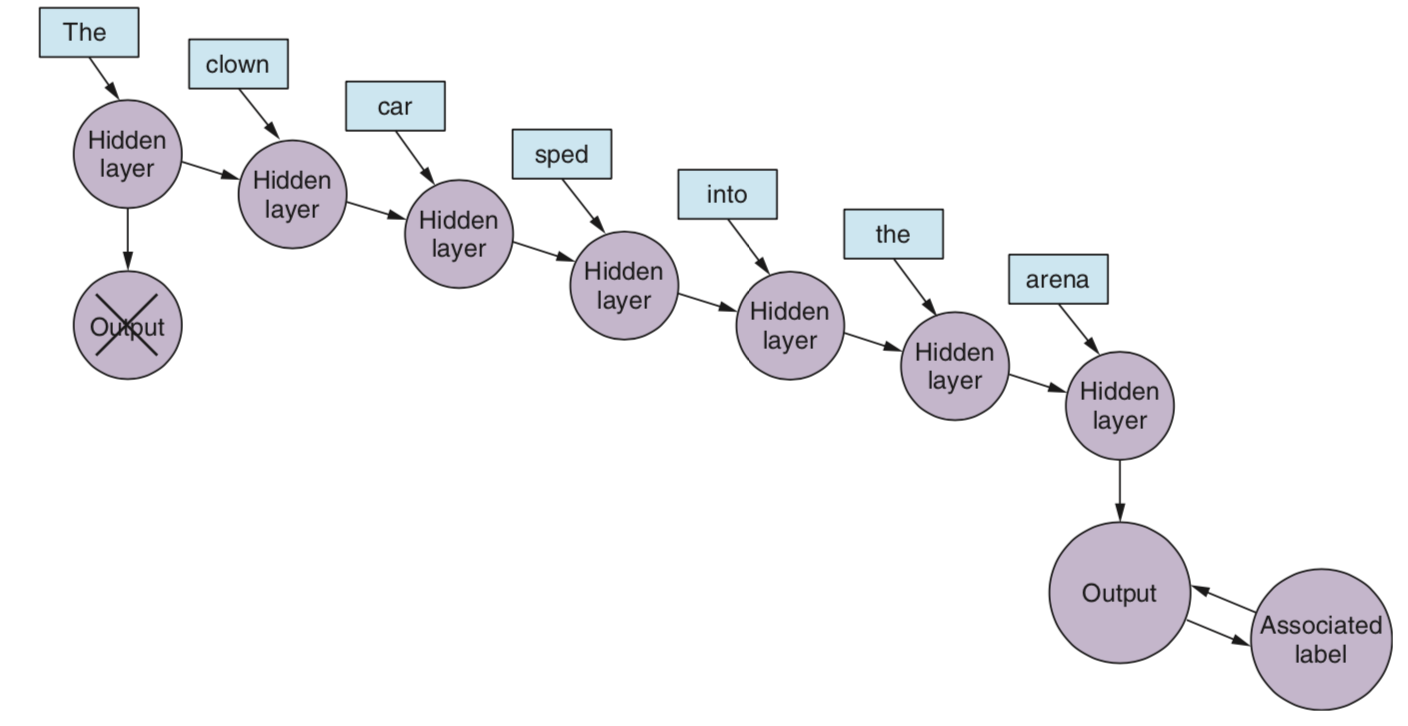
\includegraphics[width=3.4in]{figures/RNN_Flow.png}
	\caption[]{Recurrent Neural Network Model Flow} 
	\label{RNN_flow} 
\end{figure}

Figure \ref{RNN_flow} visualizes a simple RNN model flow when given the sentence “The clown car sped into the arena.” The model receives the first word “The” and creates an output. That output is hidden and carried over as an input into the model with the second word “clown”. At the third step, the model has the output from “The clown” and adds “car”. By the time we get to the end of the sentence, the recurrent neural network is able to process the entire sentence in the same order that a human would read it. This will allow the model to understand the high-level meaning of the sentence and learn the context of each word in the sentence \citep{chollet}. After the entire sentence is processed, the model is able to produce a label, sentiment, translation, response, etc. A key component of generative language models is that instead of outputting a sentiment, translation, or response, the output is the next word in the sentence. In the example above, the input would be “The clown car sped into the” and the output would be “arena”. This allows the algorithm to learn the proper way to formulate coherent sentences as it is trained on large texts. 


\subsection{Text Tokenization and Encoding}\label{token}

In order to develop a generative language model, each sentence needs to be broken down into individual units. This process is known as text tokenization. The specific unit size can vary. Depending on the model, the token may either represent a single character, a single word, group of words, or n-grams \citep{chollet}. N-gram tokens are overlapping sequenced groups of words or characters. The algorithm can only be fed numeric values in order for it to perform the mathematical calculations needed to train properly. The next step is to convert each token into a numeric vector. This process is known as encoding or embedding the text. 

For generative language models, there are two popular text tokenization methodologies. The first method is a character-level language model and the second is a word-level language model. There are many pros and cons to each methodology and the best approach depends on how the final language model is going to be used, as well as the computational constraints of the project, as word-level models have exponentially more predictive possibilities than character-level models \citep{foster}.


\subsubsection{Character-Level Language Models}\label{char}

Character-level language models tokenize and encode the individual characters in the corpus. The total number of tokens created for only letters would be 26. Each number and special character would increase the number of tokens by one.

A benefit of using a character-level language model is that the generative text output can create new words that were outside the training corpus \citep{lane}. For example, “fix” might be a word in the training corpus but “fixing”, “fixer”, and “fixed” might not. Even though the model has never seen these words, the model could easily create them because there are many other words that end with “ing”, “er”, and “ed”. The model will learn how to use these and other common character combinations in the proper way. 



\subsubsection{Word-Level Language Models}\label{word}

Word-level generative language models tokenize and encode each individual word in the corpus. The vocabulary size then becomes the number of tokens created. This can be extremely computationally expensive as there are around 20,000 common words and into the millions when including proper nouns and names \citep{lane}.


Generative word-level language model will also be unable to use any words that are outside the tokenized vocabulary list. However, a benefit over character level language model is that every output will be an actual word. Character level language models can spout out repeating characters or completely unreadable text. Word-level models will be easier to read.


\subsection{Generating New Text)}\label{new text}

Once there is a fully trained recurrent neural network language model, generating new text is a possibility. The model will need to be fed an existing sequence of words in order to predict the following word. Importantly, the newly predicted word will need to be appended onto the original sequence and fed back through the model to generate another word after that. This process is repeated over and over again to create new sentences.

Unfortunately, these models are not perfect and can produce incoherent or repetitive text. One way to combat this issue is by tweaking the way the model selects the outputted word. Typically, the output of the model is simply the highest predicted probability word. However, a model can be set to randomly sample the output words at the same level of the predicted probabilities. For example, if an output of the generative language model gave a predicted probability for the next word to be – 

 
 \begin{enumerate}
 \item Football  = 30%
 \item Basketball = 25%
 \item “Hockey” = “15%
 \item Soccer = 10%
 \item Baseball = 10%
 \item Other words combined probability = 10%
\end{enumerate} \\
  
Instead of just selecting “Football” because it is the highest, the model would randomly choose any of these words based on their associated probability. This process has been known to produce much better results \citep{lane}. To add even more variation to the generated text, a model can be given a temperature, or diversity, parameter that skews the probability distributions before the random sampling \citep{foster}. Higher temperature settings produce more “creative” chatbots by adding more randomness into the model but can also end up in nonsense \citep{lane}. Lower temperature settings will produce more deterministic results. It is suggested to play around with the temperature setting through trial and error as a chatbot is being developed \citep{foster}.



\section{Methodology}\label{meth}

The methodology implemented to carry out this study is as follows. Four distinct neural networks will be built to generate new tweets in the style of the chosen gambling twitter personalities. The Keras package in Python, which is built on TensorFlow 2.0, will be used to develop each of the four chatbots. Each of the models will use the same network architecture. They will all be recurrent neural networks (RNN) utilizing Long Short-Term Memory (LSTM) with these four steps:


\begin{enumerate}
 \item Input Layer – (Sequence of 20 Words)
 \item Embedding – (100 dimensions)
 \item LSTM Recurrent Layer – (256 units)
 \item Dense Output Layer – (User’s Vocabulary)
\end{enumerate} \\


The input layer for the recurrent neural networks will consist of a sequence of 20 words with the goal of the model to predict the next word (21st word in the sequence). The first observations fed into the model will be a sequence of 20 words, word 1 to word 20, and the output, or prediction, would be the 21st word. Then there will be a step forward of one word and the next sequence will start with word 2 and end with word 21 having the output as the 22nd word and so on.\\

For example – Joey Knish’s Tweet – 

\begin{quote}
    "I feel like the XFL needs to incorporate some weekday games next season. I don’t really wanna spend my weekends watching that trash, but much like weekday MACtion, you put a garbage football game on Tuesday night, and I’m ALL IN."
\end{quote}

\textbf{1st observation \textbf{input}} = “I feel like the XFL needs to incorporate some weekday games next season. I don’t really wanna spend my weekends”\\

First observation \textbf{output} = “watching” \\

Second observation \textbf{input} = “feel like the XFL needs to incorporate some weekday games next season. I don’t really wanna spend my weekends watching”\\

Second observation \textbf{output} = “that” \\

Third observation \textbf{input} = “like the XFL needs to incorporate some weekday games next season. I don’t really wanna spend my weekends watching that”\\

Third observation \textbf{output} = “trash” \\


The total number of trainable parameters will vary between each generative recurrent neural network based on the vocabulary size of each Twitter user and the sample size of the training data. Each mini batch size for the model’s training process will be fixed at 64 and the training will run for a total duration of 20 epochs. The optimization function used for all models will be the Adaptive Moment Estimation (Adam) optimizer in the Keras package with a learning rate of 0.001 \citep{adam}. The models will all conclude with a densely connected output layer using the softmax activation function. This activation function returns a predicted probability distribution for each possible output word \citep{lane}.


\subsection{Sports Betting Twitter Chatbots}\label{chat}

There will be four different chatbots built in this study. Each chatbot will experiment with various temperature levels to see which produces the most realistic tweets. In order for the different generative neural networks to assume the identity of the chosen Twitter users, there needs to be an exploratory analysis done on the input data first. The chatbots should produce outputs that follow in line with each users personality as follows. 

\subsubsection{Joseph Buchdahl (@12Xpert))}\label{buch}

Joseph Buchdahl is known as a skeptic academic. He appears to be a very intelligent and analytically minded individual within the sports betting community. He is the only user of the four who resides in the United Kingdom where sports betting has been legal and socially acceptable for many years. He is the author of three books focused on sports betting: “Squares and Sharps, Suckers and Sharks: The Science, Psychology and Philosophy of Gambling”, “Fixed Odds Sports Betting: Statistical Forecasting and Risk Management”, and “How to Find a Black Cat in a Coal Cellar: The Truth About Sports Tipsters.” He comes across as an elitist believing that it is practically impossible to prove that someone actually has a winning sports betting model. He instead believes that luck is the reason someone’s results may be above the breakeven level. It is also unclear whether or not Buchdahl actually participates in sports betting or if he simply pontificates to the masses about how their betting results are merely luck.

Figures \ref{tweet xpert} provides samples of his tweets from the training dataset. The topics, lengths, and spelling can vary dramatically from tweet to tweet making the learning task much harder for an algorithm with no sports betting domain knowledge or prior understanding of language.

\begin{figure}[!htb] \centering
	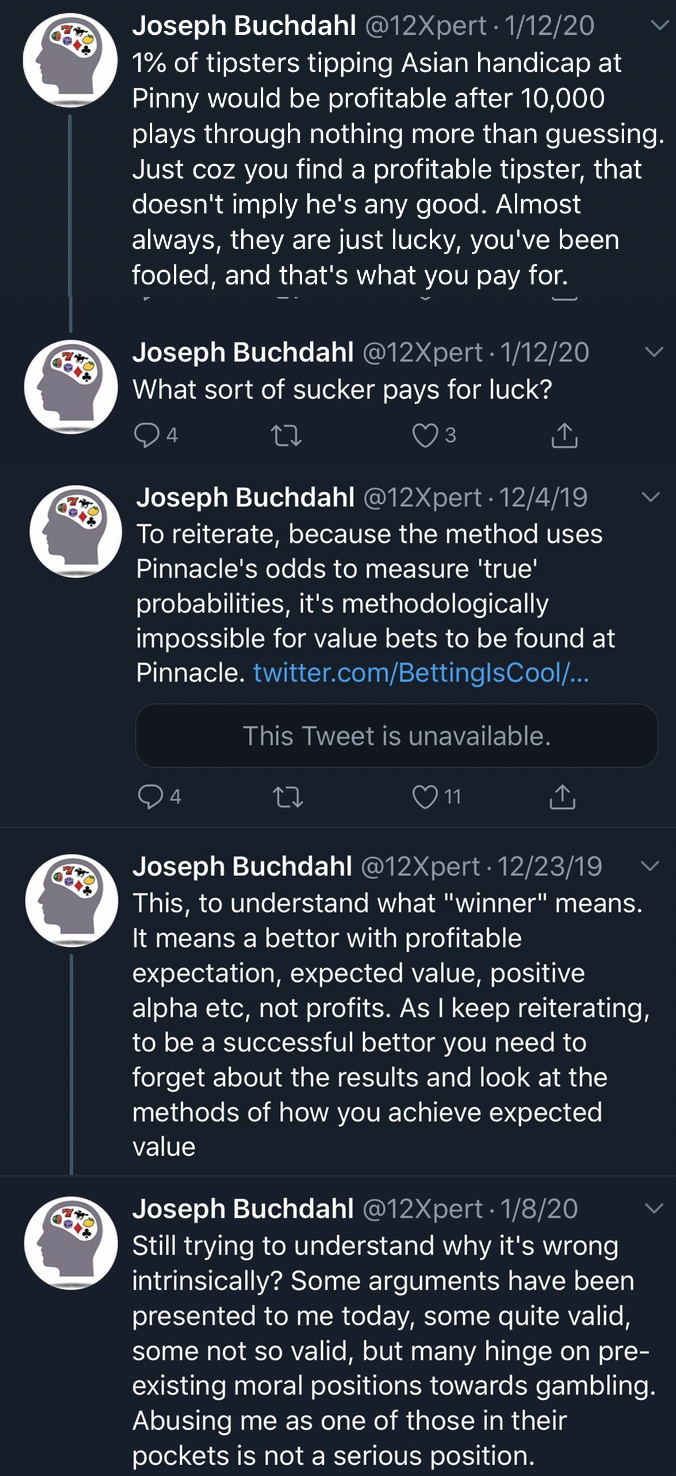
\includegraphics[width=2.0in]{figures/Tweet_Xpert.png}
	\caption[]{Sample tweets from Joseph Buchdahl's dataset showing his typical style and tone} 
	\label{tweet xpert} 
\end{figure}


An initial analysis of Buchdahl’s tweeting style is found in figure \ref{buch_personality} and is broken out into three categories \citep{Anal_words}. His emotional style strongly falls into the depressed section stemming from his constant skeptical and pessimistic tweets. Arrogance rates highest in the social style followed closely by being personable and spacy. Buchdahl’s thinking style is extremely analytical as he approaches sports betting mathematically.


\begin{figure}[!htb] \centering
	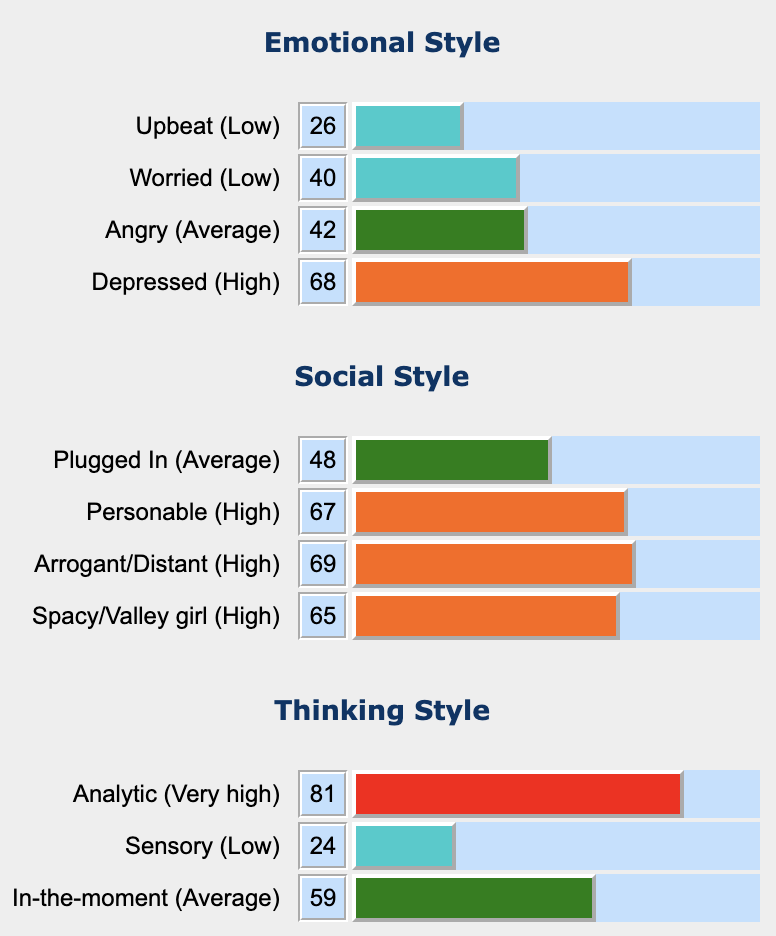
\includegraphics[width=2.5in]{figures/personality_Xpert.png}
	\caption[]{Personality diagnostics of Joseph Buchdahl’s tweets} 
	\label{buch_personality} 
\end{figure}


After the data cleaning and filtering process, there were 4,324 usable tweets from Joseph Buchdahl. His vocabulary size is 8,163 words and the number of words in all of his tweets is 126,902, with a total character count of 577,704.


\subsubsection{Joey Knish (@JoeyKnish22)}\label{knish}

Joey Knish is a fun personality and a great Twitter follow. His particular style makes him appear like your typical gambling degenerate that would blow his money betting on just about anything. His actual Twitter bio states, “Gambling Twitter Degen. Grinding that rent money. My connections run deeper than the KGB. Motor City Mouth.” Despite his degenerate appearance, he has actually been fairly successful over the years betting sports and adds his own colorful flavor to the sports betting community. He provides great insights on football and basketball, as well as in-depth analysis on the 4th of July hot dog eating contest. And yes, he does bet on people eating food and makes money doing it. He is a regular on sports betting podcasts and is always happy to talk shop with anyone interested.

Figures \ref{tweet knish} provides some sample tweets from Knish. As you can see, he can be all over the place when tweeting.

\begin{figure}[!htb] \centering
	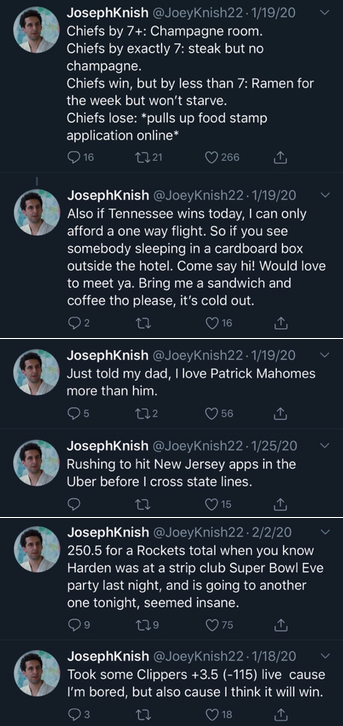
\includegraphics[width=2.0in]{figures/tweet_knish.png}
	\caption[]{Sample tweets from Joey Knish's dataset showing his typical style and tone} 
	\label{tweet knish} 
\end{figure}

Knish has a very personable tone within the sports betting community. Everyone seems to love him and his degenerative ways. As can be seen in Figure \ref{knish_personality}, he also uses language that is depressing and worried as he sweats out each bet live tweeting every emotion. He appears to be very in the moment and surprisingly analytical \citep{Anal_words}. 

\begin{figure}[!htb] \centering
	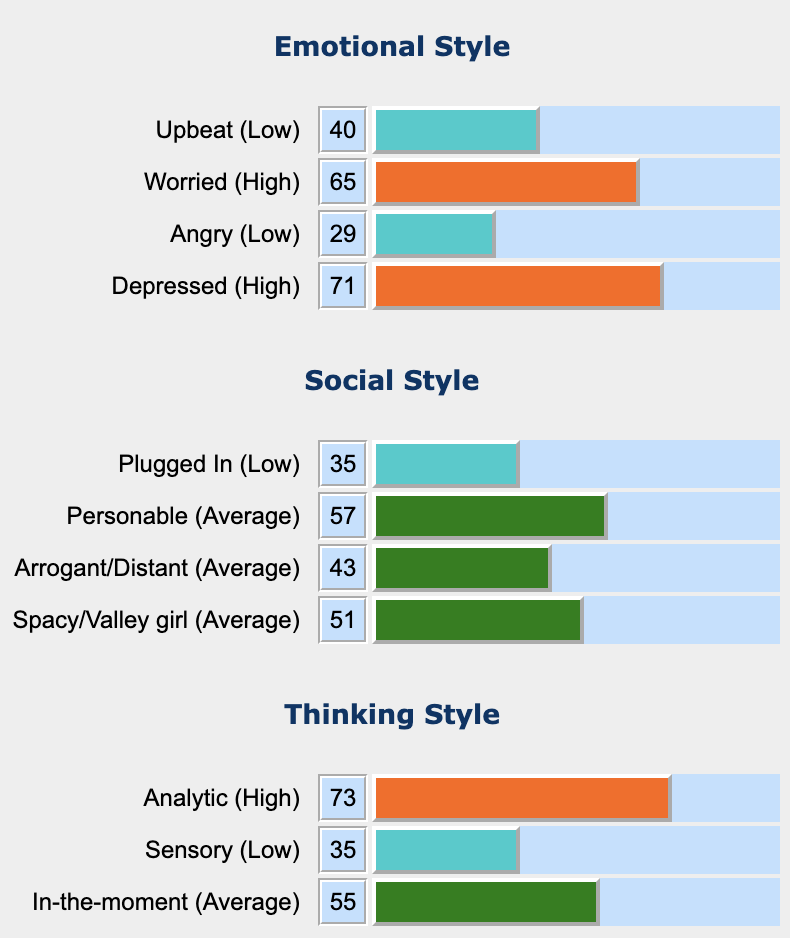
\includegraphics[width=2.5in]{figures/personality_Knish.png}
	\caption[]{Personality diagnostics of Joey Knish’s tweets} 
	\label{knish_personality} 
\end{figure}


Joey Knish’s dataset contains 4,068 tweets after the data cleansing process was completed. His vocabulary size is the greatest of all the users reaching 8,742 unique words, but 4,128 of those words only used once in the dataset. This will exponentially increase the difficulty when fitting his neural network and may need to be adjusted. There are 88,576 total words used in Knish’s dataset totaling a character string length of 378,867.



\subsubsection{Michael Schwimer (@mschwimer)}\label{swim}

Michael Schwimer is a former baseball player, spending most of his professional career in the Minor Leagues. He made a huge splash in the sports betting community last summer when he started a company called Jambos Picks. He made many outlandish claims with ridiculous guarantees. He promised his team of data scientists could deliver outrageous returns by betting sports, but you had to pay \$3,000 just to see the picks. He managed to completely unite gambling twitter in their hatred of him. He constantly talked his way in circles while never actually answering thoughtful questions and aggressively evaded any critics, even as his company failed within 5 months and discontinues selling picks, he blissfully carries on as if he is the greatest thing the sports betting world has ever seen appearing as an “Expert” on ESPN. Figure \ref{tweet swim} provides a glimpse into Schwimer’s Twitter dataset.  

\begin{figure}[!htb] \centering
	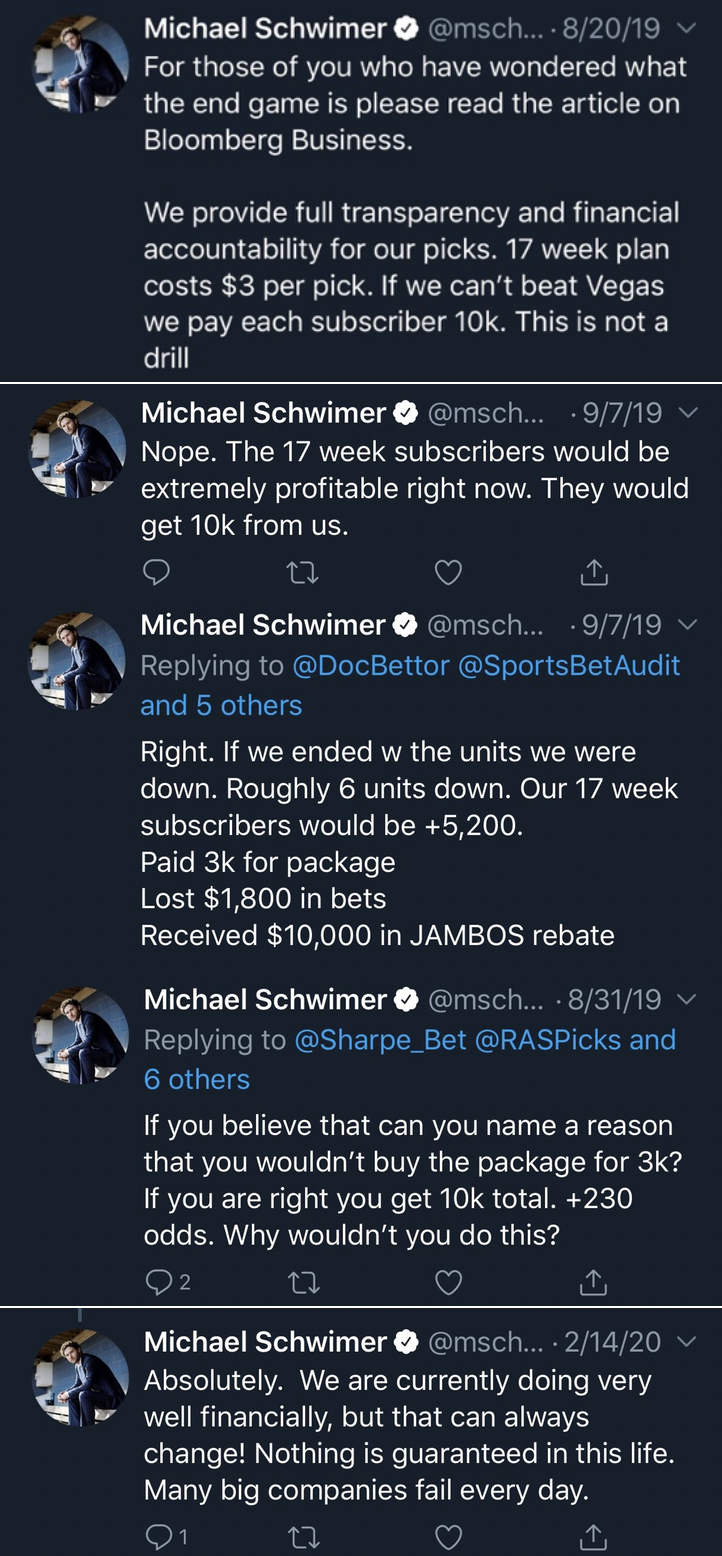
\includegraphics[width=2.0in]{figures/tweet_swim.png}
	\caption[]{Sample tweets from Michael Schwimer's dataset showing his typical style and tone} 
	\label{tweet swim} 
\end{figure}

An initial analysis of Michael Schwimer’s tweeting style is found in figure \ref{swim_personality} broken out into three categories \citep{Anal_words}. Unsurprisingly, his tweets showed an upbeat attitude coupled with a high score in the arrogant/distance category as he tried to be a salesman to the masses. He constantly tweeted out many data science buzzwords and tried to promote his company as a leader in sports analytics over the last year making his analytics thinking category very high.

\begin{figure}[!htb] \centering
	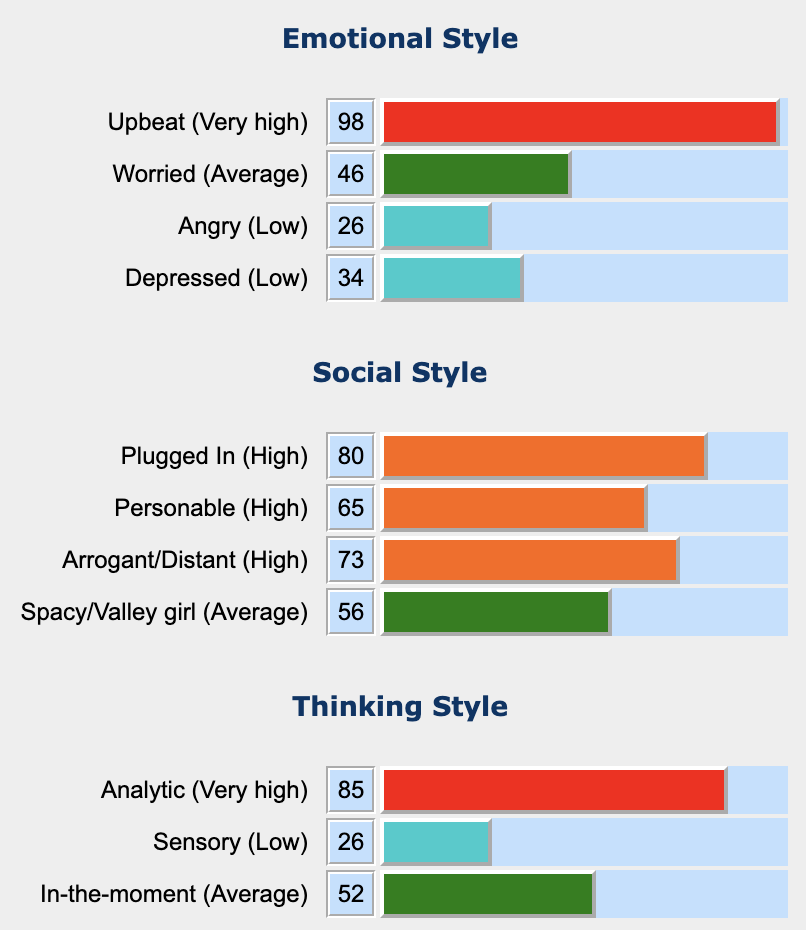
\includegraphics[width=2.5in]{figures/personality_Swim.png}
	\caption[]{Personality diagnostics of Michael Schwimer’s tweets} 
	\label{swim_personality} 
\end{figure}

After the data cleaning and filtering process, the dataset contains 2,557 tweets from Michael Schwimer. His vocabulary size is 5,010 words. There is a total of 55,540 words in his training dataset with a total character length of 227,884. 

\subsubsection{Pikachu Bets (@PikachuBets)}\label{pika}

Pikachu has a reputation as a sarcastic and angry advantage sports bettor who enjoys viciously exposing frauds and touts in the sports betting community. His tactics may be very childish and very vulgar but his commitment to honesty in a community rife with liars is commendable. Pikachu typically bets into the smaller market sports where there are more opportunities for positive expected value bets by using focused analysis. His favorite sports betting markets include obscure European soccer leagues, the Ivy league men’s and women’s college basketball, Football Championship Subdivision (formally division I-AA college football), Canadian Football league, and the WNBA. Figure \ref{tweet pika} provides samples of tweets from Pikachu’s training dataset.

\begin{figure}[!htb] \centering
	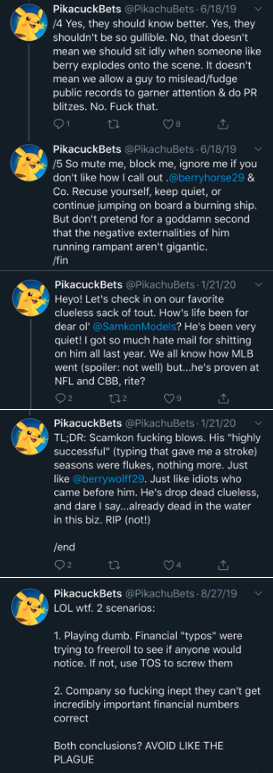
\includegraphics[width=2.0in]{figures/tweet_pika.png}
	\caption[]{Sample tweets from Pikachu's dataset showing his typical style and tone} 
	\label{tweet pika} 
\end{figure}


An initial analysis of Pikachu’s tweeting style is found in Figure  \ref{pika_personality} broken out into three categories \citep{Anal_words}. As mentioned and seen above, he scored high in the angry category. He is plugged into the community and is very personable to people unless you are caught lying or cheating. Like all of the other users, Pikachu scored high with thinking analytically. 


\begin{figure}[!htb] \centering
	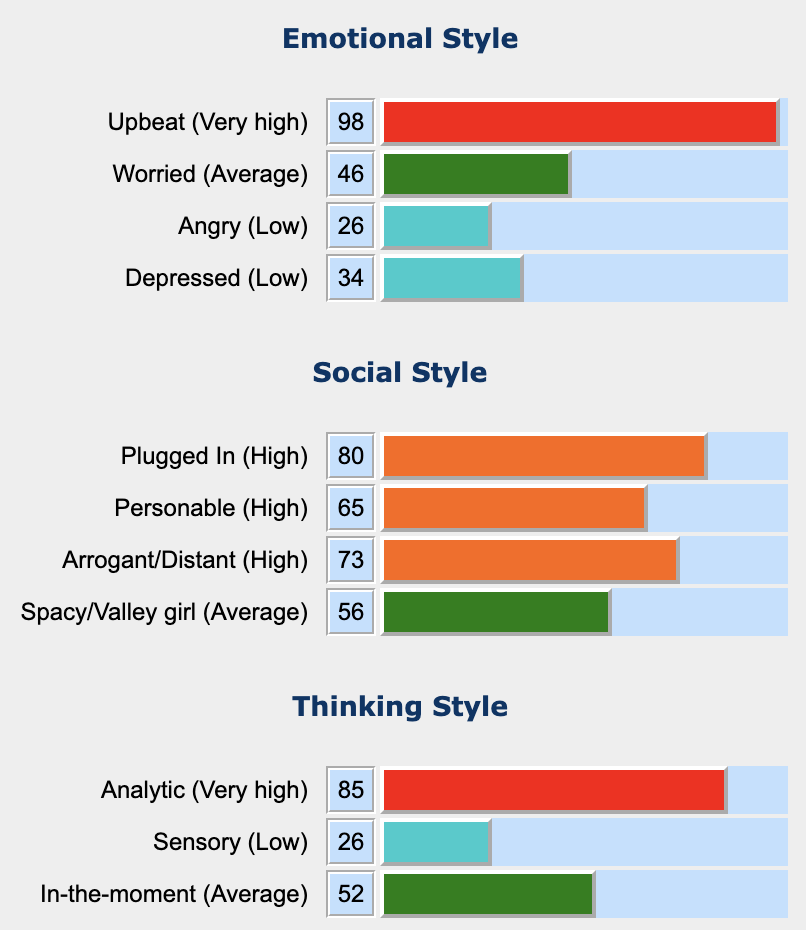
\includegraphics[width=2.5in]{figures/personality_Swim.png}
	\caption[]{Personality diagnostics of Pikachu’s tweets} 
	\label{pika_personality} 
\end{figure}


Pikachu’s dataset contains 3,047 tweets after the data cleansing process. His vocabulary size has 7,195 unique words. There is a total of 66,254 total words with a total character length of 283,219. 


\subsection{Dataset}

The complete dataset, obtained from A.I. Sports, contains 17,321 total tweets from the four chosen users operating in the gambling Twitter-sphere. There were many tweets that only contained a handful of words. These short tweets did not provide enough information to add value in the neural networks. Any tweet with six or less words were removed from the dataset leaving 13,996 valuable tweets for the algorithms to extract information from. The date range for these tweets is within the last year, March 2019 to March 2020.

Each chatbot will use only tweets from the Twitter user it is built to personify. Overfitting on the training data is not as troublesome with this type of generative neural network, meaning there will be no reason to have a hold-out dataset to test how the model works in the real world \citep{foster}. However, there will still be a split of the data during the training process with 85\% of the data used to train the model and the remaining 15\% used to validate the model. The training and validation datasets will be randomly shuffled after each epoch to allow the model the opportunity to learn as much as possible from the data. 



\subsubsection{Input Data}

The generative language models will use a word-level tokenization and encoding methodology instead of a character-level model. This decision was made after much trial and error; the word-level language models produced more coherent results. Word-level language models have significantly more tokens creating high computational costs. The words tokenized were capped at 5,500 unique words for each user to mitigate some of these costs. 

The input data represents a sequence of 20 words from the tweets of the gambling Twitter user. The first observations fed into the model will be a sequence of 20 words, word 1 to word 20, and the output, or prediction, would be the 21st word. Then there is a step forward of one word for the next 20 word input sequence.

During data preprocessing when each user’s tweets were concatenated together creating a single thread of tweets. There was a sequence of 20 “|” characters imputed between each tweet. This was done for two specific reasons. First, it will allow the models to learn where one tweet ends and where the next tweet begins. Second, it provides a convenient seed string of characters to prompt the chatbot to generate its completely original thoughts to tweet to the world \citep{foster}.


\subsubsection{Target Data}

The target data for the recurrent neural networks will be the complete vocabulary of each Twitter user. The goal of the model will be to predict the 21st word in any given word sequence. This modeling approach is a classification problem with the number of categorical classes equaling the total number of unique words in the dataset.


\section{Computational Experiment and Results}

The entire Python code for this analysis can be reproduced using \href{https://colab.research.google.com/drive/1CdjdEu8AULUHHh4gCXqsHzZDwCDKx2Rf}{Google Notebook Link} at this url:\\

\href{https://colab.research.google.com/drive/1CdjdEu8AULUHHh4gCXqsHzZDwCDKx2Rf}{LINK HERE} \\


The Python Notebook walks through each step from importing the data, cleaning, preprocessing, training each deep neural network, and using the models as chatbots generating new tweets.


\subsection{Buchdahl’s Chatbot}

The first chatbot trained was built to mimic Joseph Buchdahl’s tweeting style. Buchdahl’s total vocabulary of 8,163 words exceeded the computational constraints set during training and was capped taking the 5,500 most frequently used words. The total number of sequences of 20 words used to train this chatbot was 233,367.

Figure \ref{Xpert Summary} provides a summary of Buchdahl’s chatbot’s generative neural network structure. The 5,500 words fed into the embedding layer with 100 dimensions created 550,000 trainable parameters. Flowing through the RNN layer with 256 LSTM units created another 365,568 trainable parameters. Finally, the densely connected output layer to the 5,500 possible prediction words generated an additional 1,413,500 trainable parameters making the total trainable parameters for this recurrent neural network roughly 2.33 million. This model took 1 hour 59 minutes and 18 seconds to train over the 20 epochs.


\begin{figure}[!htb] \centering
	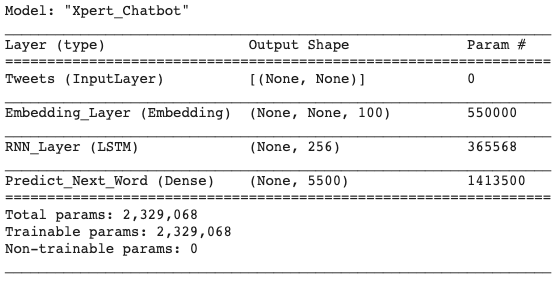
\includegraphics[width=3.4in]{figures/Xpert_Model.png}
	\caption[]{Joseph Buchdahl’s Chatbot’s Recurrent Neural Network Model Summary} 
	\label{Xpert Summary} 
\end{figure}


\begin{figure}[!htb] \centering
	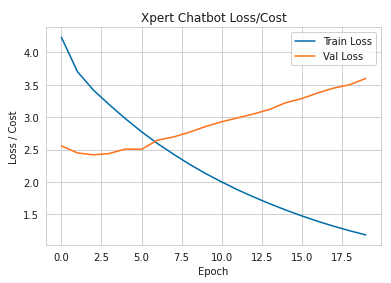
\includegraphics[width=3.4in]{figures/Xpert_Loss.png}
	\caption[]{Joseph Buchdahl’s Chatbot’s Training Loss/Cost Results} 
	\label{Xpert Loss} 
\end{figure}

\begin{figure}[!htb] \centering
	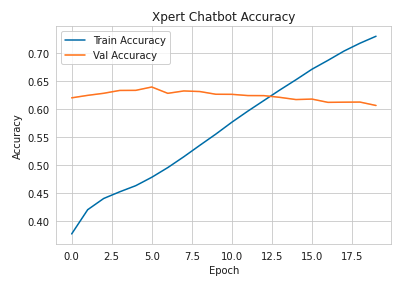
\includegraphics[width=3.4in]{figures/Xpert_Acc.png}
	\caption[]{Joseph Buchdahl’s Chatbot’s Training Accuracy Results} 
	\label{Xpert Acc} 
\end{figure}


Figure \ref{Xpert Loss} and \ref{Xpert Acc} show the training loss and accuracy, respectively, over the course of the 20 epochs. The training loss metric continued to shrink and shows signs that it would continue to shrink if it were able to train for a longer amount of time, improving the final model’s ability to sound like Buchdahl. This model reached a maximum training accuracy of 73.02\% on the training dataset and minimum loss metric of 1.1833.


\subsubsection{Best Generated Tweets}

There were many generated tweets by the newly trained Xpert Chatbot that were coherent and many incoherent. A complete list of this chatbots generated tweets can be found in the Google Colab Notebok and a condensed can be found in the appendix section.\\

\textbf{Joseph Buchdahl’s Chatbot’s Best Tweets (ordered by training time):}\\

Epoch 5, temp 0.2: I would have to see the data. I would be able to make a profit.

Epoch 7, temp 0.2: I think the point is that the tipster is not a ponzi. 

Epoch 12, temp 0.5: But if you want to know about how a ponzi operates… We don’t know nothing about this sort of s***.

Epoch 14, temp 0.5: I just think that you are not sure.

Epoch 15, temp 0.2: I think we are talking about what I was trying to articulate. The standard deviation of the world is much bigger than the signal. I suspect that the log method relationship is much more likely to be addicts.

Epoch 15, temp 0.67: Yes I was cleverer.

Epoch 19, temp 0.33: I think we already knew that football analytics companies are not as good as bookmakers to care about knowing whether it is they are not.

Final Model, temp 0.2: But it's the unintended consequences that are not the slightest idea. It is a very nuanced concept.

Final Model, temp 0.4: Yes I agree that is the point. Paradox of skill starts a betting market (expected ROI) for my view. I suspect that log method will for be linearly proportional to betshare \%.

Final Model, temp 0.4: 'True' line is meaningless because its not almost random.

Final Model, temp 0.5: But you still haven't answer my original question in my mind.

Final Model, temp 0.7: It's not enough to overcome the margin.


\subsection{Joey Knish’s Chatbot}

The second chatbot trained has the exact same number of trainable parameters as the Buchdahl’s chatbot as can be seen in Figure \ref{Knish Summary}. Joey Knish’s total vocabulary was 8,413 words, which also means there was a need to trim the word count down to the more manageable number of 5,500 words. Knish’s chatbot was able to learn from 186,110 unique sequences from his tweets.


\begin{figure}[!htb] \centering
	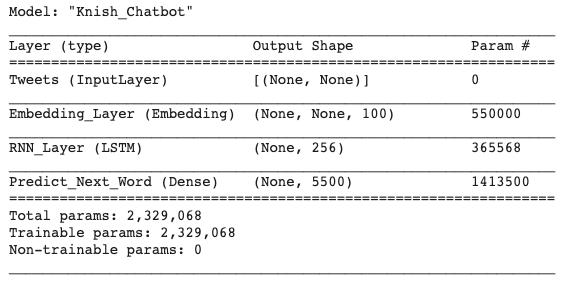
\includegraphics[width=3.4in]{figures/Knish_Model.png}
	\caption[]{Joey Knish’s Chatbot’s Recurrent Neural Network Model Summary} 
	\label{Knish Summary} 
\end{figure}


\begin{figure}[!htb] \centering
	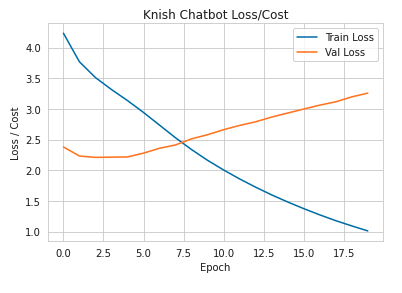
\includegraphics[width=3.4in]{figures/Knish_Loss.png}
	\caption[]{Joey Knish’s Chatbot’s Training Loss/Cost Results} 
	\label{Knish Loss} 
\end{figure}

\begin{figure}[!htb] \centering
	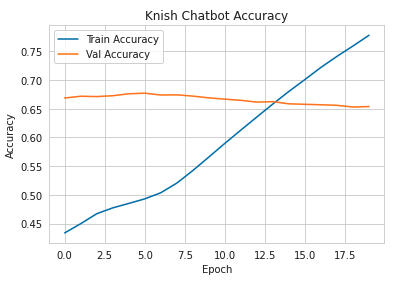
\includegraphics[width=3.4in]{figures/Knish_Acc.png}
	\caption[]{Joey Knish’s Chatbot’s Training Accuracy Results} 
	\label{Knish Acc} 
\end{figure}


Joey Knish’s chatbot was able to train in only 1 hour 21 minutes and 57 seconds, a 31\% decrease from Buchdahl’s chatbot, making it the fastest of the four recurrent neural networks trained in this study. Knish’s model was able to reach a minimum cost metric of 1.0098, Figure \ref{Knish Loss}, and a maximum accuracy of 77.79\%, Figure \ref{Knish Acc}.

\subsubsection{Best Generated Tweets}

A complete list of this chatbots generated tweets can be found in the Google Colab Notebok and a condensed list of tweets can be found in the appendix section.\\


\textbf{Joey Knish’s Chatbot’s Best Tweets (ordered by training time):}\\

Epoch 9, Temp 0.33:
The fact you’re not a delusional lunatic is not a bit surprised you can go.

Epoch 10, Temp 0.2:
I know this is fantastic. I know (lol). But I think the major trolls are legitimate. 

Epoch 13, Temp 0.5:
I thought the weekday sun belt officiating crew are solid.

Epoch 20, Temp 0.2:
Hillbillys love golf

Final Model, Temp 0.2:
I think I’m gonna stop in tomorrow night.

Final Model, Temp 0.3:
I think I bet on rutgers at halftime.



\subsection{Michael Schwimer’s Chatbot}


Michael Schwimer’s chatbot was exposed to 119,484 unique word sequences, encompassing a total vocabulary of 5,010 words. These 5,010 words flowed into an embedding layer, converting these one-dimensional tokenized words into 100 dimensions as shown in Figure \ref{Swim Summary}. This creates 501,000 trainable parameters at this stage of the model. Consistent with the other models, the following layer is a recurrent layer with long short-term memory. The LSTM layer created 365,568 more trainable parameters for the model. The 5,010 possible words that can be predicted as the output from the model are connected using a dense layer, which adds 128,7570 additional trainable parameters. Schwimer’s recurrent neural network model has approximately 2.15 million parameters that are updated during the training process. This model took 1 hour 33 minutes and 13 seconds to train over the 20 epochs.


\begin{figure}[!h] 
    \centering
	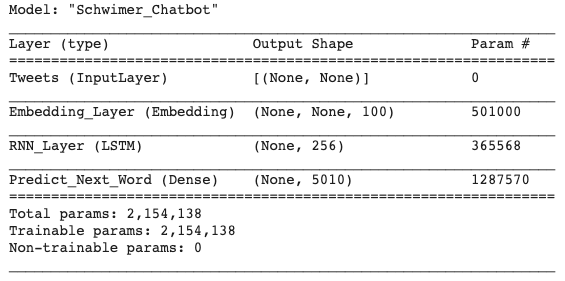
\includegraphics[width=3.4in]{figures/Swim_Model.png}
	\caption[]{Michael Schwimer’s Chatbot’s Recurrent Neural Network Model Summary} 
	\label{Swim Summary} 
\end{figure}


\begin{figure}[!htb] \centering
	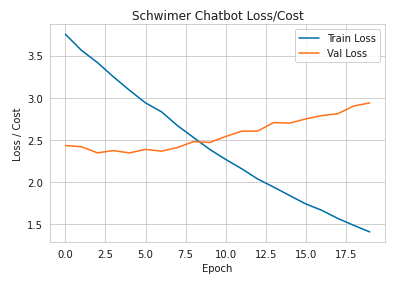
\includegraphics[width=3.4in]{figures/Swim_Loss.png}
	\caption[]{Michael Schwimer’s Chatbot’s Training Loss/Cost Results} 
	\label{Swim Loss} 
\end{figure}

\begin{figure}[!htb] \centering
	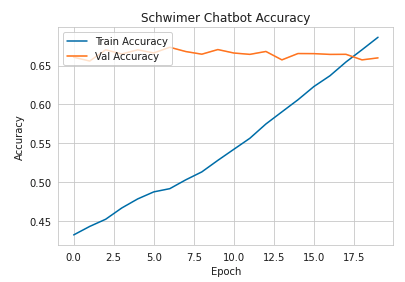
\includegraphics[width=3.4in]{figures/Swim_Acc.png}
	\caption[]{Michael Schwimer’s Chatbot’s Training Accuracy Results} 
	\label{Swim Acc} 
\end{figure}


Similar to the other models, this model continued to improve throughout the entire training process. Extending the length of time to train the model could improve the model. Figure \ref{Swim Loss} and \ref{Swim Acc} show the cost metric was the lowest in the 20th epoch at 1.4068 and the highest accuracy was found in the 20th epoch at 68.84\%.


\subsubsection{Best Generated Tweets}

A complete list of this chatbots generated tweets can be found in the Google Colab Notebok and a condensed list of tweets can be found in the appendix section.\\

\textbf{Michael Schwimer’s  Chatbot’s Best Tweets (ordered by training time):}\\

Epoch 8, Temp 0.5:
I am it! I have a lot of the Phillies Phaithful! Should be a day? 

Epoch 10, Temp 0.2:
I have not seen the truth...

Epoch 10, Temp 0.33:
I am not a problem... I have a girlfriend 

Epoch 12, Temp 1.0:
Had 101. It won 10 thousand!!!!!

Epoch 14, Temp 0.2:
I love the boss... I have nothing to hide... I have nothing to hide. 

Epoch 14, Temp 0.33:
I am not frustrated at all... 

Epoch 18, Temp 0.2:
I have not questioned a single subscriber... I have no idea... thanks for the advice and disagree. 

Epoch 18, Temp 1.0:
I’m looking for the wiz! 

Epoch 20, Temp 0.5:
This is the best week 100\% covers. we started \$2,000,000,000.

Final Model, Temp 0.2:
we have never had a 50\% chance to win. 

Final Model, Temp 0.4:
you are 100\% correct... I’m not a lot of fun... 

Final Model, Temp 0.5:
I said doesn’t mean we will be breaking the law.

Final Model, Temp 0.5:
we will be able to explain what happened. 

Final Model, Temp 0.5:
please read our detailed write up on our subscribers. they can verify our record vs. closing lines. 


Final Model, Temp 1.0:
our auditors would be surprised

Final Model, Temp 1.0:
the model is financial value. 



\subsection{Pikachu’s Chatbot}


The final chatbot trained has the same number of trainable parameters as Buchdahl’s chatbot and Knish’s chatbot as shown in Figure \ref{Pika Summary}. Pikachu’s vocabulary contained 7,195 words and needed to be reduced to only 5,500 words. There were 142,791 unique sequences created from Pikachu’s tweets that were used by the algorithm to learn Pikachu’s linguistic tendencies. This recurrent neural network was able to complete the 20 epochs in only 1 hour 9 minutes and 53 seconds making it the fastest completed chatbot in the study.


\begin{figure}[!htb] \centering
	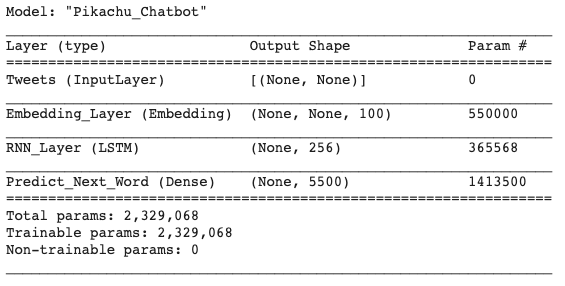
\includegraphics[width=3.4in]{figures/Pika_Model.png}
	\caption[]{Pikachu’s Chatbot’s Recurrent Neural Network Model Summary} 
	\label{Pika Summary} 
\end{figure}


\begin{figure}[!htb] \centering
	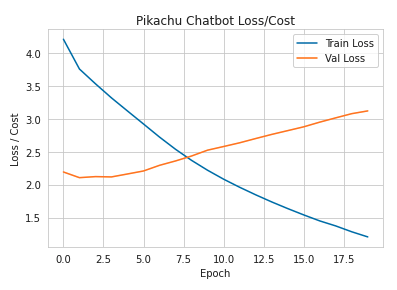
\includegraphics[width=3.4in]{figures/Pika_Loss.png}
	\caption[]{Pikachu’s Chatbot’s Training Loss/Cost Results} 
	\label{Pika Loss} 
\end{figure}

\begin{figure}[!htb] \centering
	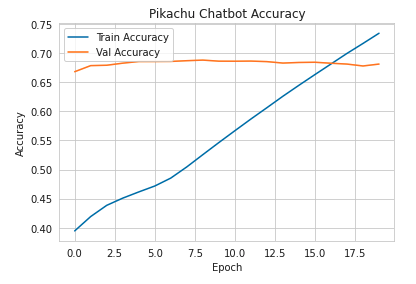
\includegraphics[width=3.4in]{figures/Pika_Acc.png}
	\caption[]{Pikachu’s Chatbot’s Training Accuracy Results} 
	\label{Pika Acc} 
\end{figure}


The training accuracy of Pikachu’s chatbot increased steadily at 1.55\% per epoch peaking at 73.39\% in the final epoch. The cost metric reached its minimum of 1.2059 in the final epoch as well. 


\subsubsection{Best Generated Tweets}

A complete list of this chatbots generated tweets can be found in the Google Colab Notebok and a condensed list of tweets can be found in the appendix section.\\

\textbf{Pikachu’s Chatbot’s Best Tweets (ordered by training time):}\\


Epoch 5, Temp 0.33:
I am a f***ing joke... 

Epoch 10, Temp 0.5:
Great humble brag. Thanks me. 

Epoch 12, Temp 0.2:
I am uber aware thank you very much. If you want to be a bozo 

Epoch 12, Temp 1.0:
10/4 NBA lockz BOS +7 .5units

Epoch 13, Temp 0.67:
Eurocup Andorra -3.5 Barcelona -8.5 China CBA Nanjing +10. 56\% ROI CLV: +0.02pt 

Epoch 14, Temp 1.0:
lol I won't owe. not me lol 

Epoch 19, Temp 0.67:
I took my time to commit a federal felony! 

Final Model, Temp 0.1:
I agree. you don’t know shit about analytics or something something 

Final Model, Temp 0.1:
I agree. you don’t know basic s*** like this... 

Final Model, Temp 0.4:
you are not a modeler....

Final Model, Temp 0.5:
They’re just coaching and playing college ball. 

Final Model, Temp 0.5:
a lot of these kids are smart. 

Final Model, Temp 0.6:
you're just a good ass liar. 




\section{Discussion and Conclusions}


\begin{table}[!htb] 
  \centering 
  \begin{tabular}{@{\small}llll@{}} 
    \toprule % utilise booktabs
    & {\footnotesize Training Time} &  {\footnotesize Loss/Cost} & {\footnotesize Training Acc} \\ \midrule
    Xpert & 1:59:18 & 1.1833 & 73.02\% \\
    Knish & 1:21:57 & 1.0098 & 77.79\% \\
    Schwim & 1:33:13 & 1.4068 & 68.84\% \\
    Pika & 1:09:53 & 1.2059 & 73.39\% \\ 
    \bottomrule
\end{tabular} \caption{Side by Side comparison of the four deep neural networks} \label{table_eval}
\end{table}


Table \ref{table_eval} compares each of the models training times, cost/loss metric, and accuracy. Buchdahl’s chatbot required the greatest amount of time to complete and Pickachu’s chatbot finished in almost half the time. While their timing was vastly different, their accuracy was nearly identical. The Knish chatbot was able to learn the most from the data and Schwimer’s chatbot learned the least.

After reviewing all of the generated tweets, the way that each model was able to learn the personality of the specific user was incredibly impressive overall. It was very clear which tweets came from which user. Another impressive feat the models accomplished that could easily go unnoticed when reviewing the chatbots’ results was their ability to learn proper sentence structure and how to use quotation marks and parentheses. Many of the generated tweets were complete sentences with a period at the end. The models also used “…” correctly and other punctuation. There were words that were used sarcastically by the model and the model knew that it should use quotation marks on both sides of the word just like a human would do. There were also many times where parentheses were used correctly with an opening and closing parenthesis. This is only possible because the recurrent neural networks are able to remember what words or punctuation came earlier in the sentence enabling them to appropriately learn their uses.

Potential future work to improve the realism of these chatbots would include increasing the sample size significantly giving the models more data to learn. Another improvement would be to allow the recurrent neural networks to train for a significantly longer time. This study was very limited because of the hardware available, but a future study could utilize virtual machines with the models trained in the cloud with multiple GPUs or TPUs. Each model was showing signs that it would continue improving with more training time.

Fine tuning hyperparameters, increasing the number of layers, or increasing the number of neurons in each layer may garner improved performance of the chatbots. All of these things can help decrease the number of incoherently generated tweets and increase the chatbots ability to sound human.

In conclusion, the primary goals of this study were accomplished. Four generative deep learning models were built to create new tweets taking on the persona of Joseph Buchdahl, Joey Knish, Michael Schwimer, and Pikachu Bets respectively. Adjusting the temperature of the predicted probability distribution for each word allowed the chatbots to become more creative and realistic. Generative recurrent neural networks models with long short-term memory are powerful algorithms and appropriate to use when building realistic chatbots.


\clearpage

\appendix{Appendix}\label{Appendix}

{}\\
  
\textbf{Tweets:}\\


\textbf{Joseph Buchdahl’s Chatbot’s Tweets (ordered by training time):}\\

Epoch 3, temp 0.2: “I think you know that the bookmaker is a lot of the market.”

Epoch 4, temp 0.33: “New predictions for 2019-20 (method at including fixture difficulty and more). Attack strength defence weakness ratings shown by team. Data by”

Epoch 4, temp 0.67: “It seems to be considered a behavior of skin and the latter is not restricted for their numbers. It is not a real thing.”

Epoch 5, temp 0.2: “I would have to see the data. I would be able to make a profit.”

Epoch 6, temp 0.33: “I don’t doubt they are. I don’t think it is that the bookmaker is because they are not!”

Epoch 7, temp 0.2: “I think the point is that the tipster is not a ponzi. If you can do it?”

Epoch 7, temp 0.33: “If you’re talking about the data to prove that the closing price is not efficient. I don’t know what I find it.”

Epoch 7, temp 0.67: “I know I know… I can see that it would be 100,000”

Epoch 8, temp 0.2: “I think the point is that the question is that the proportion of the big boundaries is that the law of the vig is not quite enough to be addicts.”

Epoch 8, temp 0.33: “I think the answer is that the closing price is a lot of the margin. But I think it didn’t apply the data.”

Epoch 8, temp 0.5: “I think it’s conflating the problem with one of the bookmaker? That would be a special case.”

Epoch 9, temp 0.2: “I don’t doubt that I don’t know. I don’t know what the closing line value is not the same.”

Epoch 9, temp 0.67: “I don’t believe it’s a strong case for why I can do It all. But I don’t need to use it.”

Epoch 10, temp 0.2: “I think the argument is that the standard deviation is that the proportion of the vig shifted.”

Epoch 12, temp 0.2: “I think the point is that the of the time is that they are. And if you think that they are puzzled why they don’t want to be wrong.”

Epoch 12, temp 0.5: “But if you want to know about how a ponzi operates… We don’t know nothing about this sort of shit.”

Epoch 13, temp 0.2: “I think the argument that I think it is a duck swims like a duck and quacks like a duck. I think most people who think it is to be fooled by randomness.”

Epoch 13, temp 0.33: “I don’t care that I don’t agree with you. I’m not saying that was a story. But I don’t think I don’t like the data.”

Epoch 13, temp 0.5: “Well I think the point is making a lot of bs.”

Epoch 13, temp 0.67: “My hunch is a simple measure of advantage but as with his tipster it’s a significant extent value but the fact that they don’t want to lose.”

Epoch 14, temp 0.2: “I think the point is that the biggest stakers were the potential to be winning. But if you are unable to beat pinnacle.”

Epoch 14, temp 0.33: “I guess the odd are the 1,035 matches from 1,777 bets variable odds that is the same. It gets bigger than 1.55.”

Epoch 14, temp 0.5: “I just think that you are not sure.”

Epoch 15, temp 0.2: “I think we are talking about what I was trying to articulate. The standard deviation of the world is much bigger than the signal. I suspect that the log method relationship is much more likely to be addicts.”

Epoch 15, temp 0.67: “Yes I was cleverer.”

Epoch 16, temp 0.5: “I think you’re not something that worked and non-doping is statistically good at a nation to think that it was.”

Epoch 18, temp 0.5: “I think the argument from the pleasure gained bring via the anticipation of uncertain and not human day. It has a little on a bit of gambling addiction.”

Epoch 18, temp 0.67: “I’m not asking him to care about luck. If you hate me then we don’t seem to be! “Everyone” they’re so you just have nothing constructive to make it anymore.”

Epoch 19, temp 0.33: I think we already knew that football analytics companies are not as good as bookmakers to care about knowing whether it is they are not.

Epoch 20, temp 0.5: It’s a good thing. Do you think they are blind to point out how you achieve so right?

Final Model, temp 0.2: If you mean they wouldn't be fully efficient but they can be errors in the end why would anyone pay me to embark on your own bookmaker. We think this is the case that man city thought have been used in the original time.

Final Model, temp 0.2: But it's the unintended consequences that are not the slightest idea. If it is a very nuanced concept.

Final Model, temp 0.3: But you still haven't shown for the two data i.e. comparing into your turnover and see average.

Final Model, temp 0.3: I know I know. The point is that if it was the way to make a living from betting companies.

Final Model, temp 0.4: You don't know. I don't know how much I would have to do to be betting or more than they do so.

Final Model, temp 0.4: Yes I agree that is the point. Paradox of skill starts a betting market (expected ROI) for my view. I suspect that log method will for be linearly proportional to betshare \%.

Final Model, temp 0.4: I would say shame that if you know what the amount you know. 'True' line is meaningless because its not almost random.

Final Model, temp 0.5: But when I think it's a scam it's chapter 10 years. But she will be a negative yield and difference. We have to talk about this.

Final Model, temp 0.5: But it's the unintended consequences that are not the point. Best if indeed it offers you are useful anyway.

Final Model, temp 0.5: But you still haven't answer my original question in my mind. And the long term it would be more efficient than other than the vig and how many are close.

Final Model, temp 0.6: This is just an obvious reality. I haven't noticed. I have to read the piece if we consider doing this truth. If you read the view that this is the same thing and the only thing for that they are and managing risks. That is why you might not be talking to the true probability that it might explain why.


Final Model, temp 0.7: You will but you have to be suggesting we wouldn’t see the problem of "winners" to make it better because of this privately and my majority are socioeconomically able to pass in.

Final Model, temp 0.7: I would say shame that the reason all for skilled records is about 99\% who are in-year. It's not enough to overcome the margin. 

Final Model, temp 0.7: I didn't say I would say that is a decent point and go nuts. But has yet been banned by the paradox of sharp bettors. 

Final Model, temp 0.7: If you mean market efficiency or you are more than 1\%. You would need to lose a bonferroni correction. Here's a p-value where -4 knowing how you don't have the data shut to change your expected.

Final Model, temp 0.8: A blog agree to know how a reason to say "model" to retag and knowledge particularly about allowing who that is bringing to the market you exploit it.

Final Model, temp 0.9: I think this is the common different moral of the cycle that sees moral attitudes to gambling flip. There will be anything else to achieve that there are other reasons?

Final Model, temp 0.9: Week your bayes factor punters for fivethirtyeight there are not perfectly efficient at least that is what you are.


Final Model, temp 1.0: The only place is whether were a coin flipper with a big records which can't happen to be verified with that you will get access to luck goal.\\


\textbf{Joey Knish’s Chatbot’s Tweets (ordered by training time):}\\

Epoch 6, Temp 0.2:
But I think the guy is a great fan. 

Epoch 6, Temp 0.33:
I think the guy is a great guy.

Epoch 8, Temp 0.2:
I think the guy is a great advisor to the trap maize and don’t want to overreact. 

Epoch 9, Temp 0.2:
I think the owner is a fantastic. But the guy is a great speech. 

Epoch 9, Temp 0.33:
The fact you’re not a delusional lunatic is not a bit surprised you can go. 

Epoch 10, Temp 0.2:
I know this is fantastic. I know (lol). But I think the major trolls are legitimate. 


Epoch 10, Temp 0.33:
I just thought he was gonna be a true punch you. So I guess. 


Epoch 11, Temp 0.33:
I don’t think he’s fully healthy.


Epoch 11, Temp 1.0:
cash ppl haven’t spent oddsmaker secret again. You’ve got it baby.

Epoch 12, Temp 0.2:
I think the guy were gonna be a rough delta between the new trenches and 2,000.

Epoch 12, Temp 0.33:
I like how akron recruited 5 thousand in football.

Epoch 13, Temp 0.5:
I thought the weekday sun belt officiating crew are solid.

Epoch 14, Temp 0.5:
I love the parlays where they got up and cleaned

Epoch 15, Temp 0.67:
The XFL is gonna send him a lot of ppl that bet looks like that are on the daily tees. 

Epoch 16, Temp 0.2:
I know you took a bunch of juice before but I think he’ll do a ton of money. 

Epoch 16, Temp 0.33:
Hopefully that is gonna overreact. But would likely be a handful of people. 

Epoch 16, Temp 0.5:
I don’t think its fixed. but is something.

Epoch 17, Temp 0.2:
I think the funnier part is actually I agree with the future room.

Epoch 17, Temp 0.33:
I think one of my favorite of my guys on a football and they don’t need to kill myself with a segment. 

Epoch 17, Temp 0.67:
I think TJ Watt + 900 a month after a 9 month. 

Epoch 17, Temp 1.0:
uncle knish may got a small 10.5 tries +81 a month 

Epoch 18, Temp 0.2:
I don’t think that is much more popular but had me a good sized good ham to this summer.

Epoch 19, Temp 0.5:
If you need me, I’ll be checking prices as a 10 min for a late cash and I’ll be tough to the local props. 

Epoch 19, Temp 0.67:
He’s hedge there like a clue. There’s never been a great group 

Epoch 19, Temp 1.0:
That’s I just can’t think about that really don’t see the sports twitter 

Epoch 20, Temp 0.2:
Hillbillys love golf

Epoch 20, Temp 0.33:
I think it’s official. The touts have really made a great bag of the future before I have a 3\% on that that in the world cup. 

Epoch 20, Temp 1.0:
Somebody knows. Don’t do \$20 bucks. 


Final Model, Temp 0.1: 
I like this game. 

Final Model, Temp 0.1: but it’s not too much at the conference and a prize week. 

Final Model, Temp 0.2: 
I think I’m gonna stop in tomorrow night.

Final Model, Temp 0.3: 
I think I bet on rutgers at halftime.

Final Model, Temp 0.3: if you have a dm to go up to stay and get the knishwich up 8.

Final Model, Temp 0.3: I think I’m gonna drive franky lol but never been a couple of it 4th but didn’t get the line. 

Final Model, Temp 0.3: I think it’s official. the touts can be a shot. great list (tampa) even in detroit 

Final Model, Temp 0.4: 
12-19 conference title games that is going into power ratings.


Final Model, Temp 0.4: I think the guy was also too much too.

Final Model, Temp 0.5: 
that moment when you go to your non / walk for 258 million?

Final Model, Temp 0.5: the hospital horror stories + lack of supplies in epicenter areas is bad. real bad

Final Model, Temp 0.5: you know if benny is dunking on ya on the al world.

Final Model, Temp 0.5: I think I would have to do this.

Final Model, Temp 0.5: also probably not got the best qb in the house in the country.

Final Model, Temp 0.5: I think you should stop in the game but the part of the next game. 

Final Model, Temp 0.6: 
but nobodys got a personal soccer play in the night

Final Model, Temp 0.7: 
nah if you DM’d matt not a reality of his knowledge probably be fine. 

Final Model, Temp 0.7: A MAC coaching staff not realizing the bears

Final Model, Temp 0.7: 4.5 which was a good time for him to justify what just the quick or get some prop.

Final Model, Temp 0.8: 
I would imagine you’re the old man of gambling

Final Model, Temp 0.8: if you ride a nice jersey and dm it can cheap then a cover 

Final Model, Temp 0.8: Penny don’t think shit.

Final Model, Temp 0.8: lmao not 500\% sure I tried to get in the last 20 points her
feels like you’re bordering on ben 

Final Model, Temp 0.9: 
I think 6 of the last 15 hours with the greatest lead and MLB football return.

Final Model, Temp 0.9: you know tickets are an option I’ve got it

Final Model, Temp 1.0: I just won a few rd. you just never won a winner.

Final Model, Temp 1.0: yeah he’s gonna run

Final Model, Temp 1.0: thanks for cleaning it taking the strip today to give it back\\




\textbf{Michael Scwhimer’s Chatbot’s Tweets (ordered by training time):}\\

Epoch 8, Temp 0.5:
I am it! I have a lot of the Phillies Phaithful! Should be a day? 

Epoch 9, Temp 0.5:
I think you can pay you can discuss. If you have a lot of our subscribers... I have a lot of the game and I will be able to win. 

Epoch 10, Temp 0.2:
I have not seen the truth...

Epoch 10, Temp 0.33:
I am not a problem... I have a girlfriend whom I have no idea 

Epoch 10, Temp 0.67:
We don’t think market. Never say we did... We have a units calculator for our subscribers. 

Epoch 11, Temp 0.2:
I have not questioned a single reason you can bet the market consensus line than the game. If you are right. 


Epoch 11, Temp 0.33:
we are not a bad... I have a girlfriend whom I have pursued.... 

Epoch 12, Temp 0.2:
I am not frustrated at the game of the Phillies... I love to be the king of the game 

Epoch 12, Temp 0.5:
it is 100\% agree... I have always beaten me... I’m hurt... 

Epoch 12, Temp 1.0:
Had 101. It won 10 thousand!!!!!

Epoch 13, Temp 0.5:
If you don’t believe that then we are doing 10 thousand. But if you wouldn’t do whatever they want. 

Epoch 14, Temp 0.2:
I love the boss... I have nothing to hide... I have nothing to hide. 

Epoch 14, Temp 0.33:
I am not frustrated at all... 

Epoch 15, Temp 0.5:
Again! I am a 100\% agree... it is not a good... I have no idea it is a great platform... I have no idea. 

Epoch 15, Temp 0.67:
I have 100\% agree with a girl not certainly up all our stuff. 

Epoch 16, Temp 0.2:
I have a solution to the sixer loss... 
I think I was gonna be hooked on ur dorm group 

Epoch 17, Temp 0.2:
I think it is gonna be on ur twitter bio to warrant a XXL hoodie 

Epoch 18, Temp 0.2:
I have not questioned a single subscriber... I have no idea... thanks for the advice and disagree. 

Epoch 18, Temp 1.0:
I’m looking for the wiz! 

Epoch 19, Temp 0.33:
I am not a fan... I love it as a good...

Epoch 19, Temp 0.5:
I have been trying to scam but I have heard a good thing about him 

Epoch 19, Temp 0.67:
Why is CNN not me... It’s a big fine.... if it came into me... 

Epoch 19, Temp 1.0:
That wasn’t a true. Steve always tweet by fun as well!


Epoch 20, Temp 0.5:
This is the best week 100\% covers. we started \$2,000,000,000.

Epoch 20, Temp 0.67:
We have lots of thoughts and have doing super email that when we have a problem with any questions because I consider not not clear. 

Final Model, Temp 0.1: 
I have a venmo account that proves I have told me every single world. I have no athleticism to compete. 

Final Model, Temp 0.1: 
I am not frustrated at all... I love to baptize the stuff on ur salon

Final Model, Temp 0.2:
No. We are currently able to pay you +230 units on our fee. 

Final Model, Temp 0.2:
I am not frustrated at all... I have always seen the game though... 

Final Model, Temp 0.2:
we have never had a 50\% chance to win. 

Final Model, Temp 0.2:
I have not questioned any of the jambos. I have no idea... thanks for the advice. 

Final Model, Temp 0.3:
we are not dealing with that. we have a units calculator on our site 

Final Model, Temp 0.4:
you are 100\% correct... I’m not a lot of fun... I’m not nearly signing up. 

Final Model, Temp 0.5:
I said doesn’t mean we will be breaking the law.

Final Model, Temp 0.5:
we will be able to explain what happened. 

Final Model, Temp 0.5:
they have a lot of respect and what they have.

Final Model, Temp 0.5:
why would you accept money by how we define money?

Final Model, Temp 0.5:
please read our detailed write up on our subscribers. they can verify our record vs. closing lines. 

Final Model, Temp 0.5:
yes. do you get it from your money?

Final Model, Temp 0.5:
if you are missing something you say you are right, you get 100 thousand if you are wrong. 

Final Model, Temp 0.6:
It’s a bad start! I’ve been a lot of fun at each half? I'm the top 2

Final Model, Temp 0.6:
if you don’t believe that then put your money where your mouth is. we are giving you! 

Final Model, Temp 0.7:
I have no smart win in football...

Final Model, Temp 0.8:
good. and will you recommend the birthday wishes. especially about the sweet present. 

Final Model, Temp 0.8:
our plan covers the very tough to game... 

Final Model, Temp 0.9:
will review everything on the jags / titans game 

Final Model, Temp 1.0:
our auditors would be surprised

Final Model, Temp 1.0:
that is not fair bs.

Final Model, Temp 1.0:
I don’t take the same for a financial cat.

Final Model, Temp 1.0:
the model is financial value. \\




\textbf{Michael Scwhimer’s Chatbot’s Tweets (ordered by training time):}\\




Epoch 5, Temp 0.33:
I am a fucking joke... 

Epoch 5, Temp 0.5:
Wow you have a fucking name. But a tout is a guy lol 

Epoch 6, Temp 0.2:
10/20 ivy CBB madness add -110.5 -10.5 

Epoch 8, Temp 0.33:
I agree I didnt owe anyone. 

Epoch 8, Temp 0.67:
I'm trying to do the full package?????? 

Epoch 10, Temp 0.33:
I agree...

Epoch 10, Temp 0.5:
Great humble brag. Thanks me. your company is a direct quote in the day. 

Epoch 10, Temp 0.5:
he is the problem with this wk 100 on the season 

Epoch 11, Temp 0.5:
no. I just suggested your name / affiliate packages 

Epoch 12, Temp 0.2:
I am uber aware thank you very much. If you want to be a bozo 

Epoch 12, Temp 0.5:
you sound like no. if you think he is not a modeler...

Epoch 12, Temp 1.0:
10/4 NBA lockz BOS +7.5 units

Epoch 13, Temp 0.67:
Eurocup Andorra -3.5 Barcelona -8.5 China CBA Nanjing +10. 56% ROI CLV: +0.02pt 

Epoch 14, Temp 0.5:
lol I don't want to get the job quoting lines 

Epoch 14, Temp 1.0:
lol I won't owe. not me lol 
Epoch 15, Temp 0.2:
you know you can get the stipend in the business who all those plays??? 

Epoch 15, Temp 0.33:
we can bet $10 thousand ez-pz when you charge $100 on his $5000? do you recommend your $500

Epoch 15, Temp 0.67:
he said this first year at our trading desk.

Epoch 16, Temp 0.33:
10/22 ivy CBB 307827 Princeton -1. 58% ROI CLV: +0.45pt 

Epoch 16, Temp 0.67:
found a draft every year realizing I cap off of the tournament. this is the same and they are even close 

Epoch 16, Temp 1.0:
what me was it? what the conference amounts to rate a gambler.

Epoch 17, Temp 0.2:
lol you are you a guy who commented on sports about being a tout bettor. he paid out you didn't

Epoch 17, Temp 0.33:
lol you know this whole twitter fallacy. you realize the probability of the worst degens casino like a lot. bozo 

Epoch 17, Temp 0.5:
lol this is a fucking life. no I didnt know shit about sports finances.

Epoch 17, Temp 0.67:
This is just a dime a dozen meatheads long as opposed to the pp pages. 

Epoch 18, Temp 0.5:
11/14 ivy CBB 741 Penn -3.5 season: 17-11. 56% ROI CLV: +0.12pt 

Epoch 18, Temp 0.67:
legit. imagine being a hard to book when you are it at all. I leave him for names he was doing.

Epoch 19, Temp 0.33:
if you think a market exists 1.5! or are you a great start 

Epoch 19, Temp 0.67:
I took my time to commit a federal felony! 

Epoch 20, Temp 0.2:
10/20 NBA PHI u212.5 UTA u210.5 season: 21% ROI CLV: 1-12-1. fuck me. 

Epoch 20, Temp 0.33:
11/27 ivy CBB 783 Yale +13 season: 1-1-1 

Epoch 20, Temp 0.67:
if you tweeted a tout and now where he did all the time to say just say you are not a fan? 

Epoch 20, Temp 1.0:
imagine being a professional football team and guess and you tweeted posting a goal to the international community then simply keep playing my own 

Final Model, Temp 0.1:
lol. visit queens. it's not even funny the data 

Final Model, Temp 0.1:
this is not a fucking difficult concept to outs. you are missing the sharp stuff he's been out 

Final Model, Temp 0.1:
I agree. you don’t know shit about analytics or something something 

Final Model, Temp 0.1:
I agree. you don’t know basic shit like this... 

Final Model, Temp 0.1: you still wanna be profitable about the phone ty " I don't want to admit it 

Final Model, Temp 0.2:
but wait you have vastly underperformed all down with the finish 

Final Model, Temp 0.2:
I am uber aware tyvm. why are you obsessed with dicks 

Final Model, Temp 0.2:
I don't see this game or something. it wasn't a pro and reliable. zero..

Final Model, Temp 0.3:
I don't want to get ahead of shit except memes " 

Final Model, Temp 0.3:
no vig reverse sweep then sweep then reverse sweep again last 3 years 

Final Model, Temp 0.4:
you are not a modeler....

Final Model, Temp 0.5:
I don't get shit. prob just retire in february but I just thought it all and prove to work? 

Final Model, Temp 0.5:
They’re just coaching and playing college ball. 

Final Model, Temp 0.5:
Shouldn’t be able to get down with your ivy league public 

Final Model, Temp 0.5:
a lot of these kids are smart. 
Final Model, Temp 0.6:
wnba " is a fucking bullshit argument " you listen to a tout

Final Model, Temp 0.6:
you're just a good ass liar. 

Final Model, Temp 0.8:
millions on no surprise he thinks guys going to be an edge. also are still hate here

Final Model, Temp 0.9:
your big is to talk about shit so strong. you are just a short-time.
5 got +5.5 -19.5 good good

Final Model, Temp 1.0:
might sprinkle some steam and deleted all of them. 

Final Model, Temp 1.0:
no but it was the target audience to play for it used to $2-0 thousand 

Final Model, Temp 1.0:
to lose probably and w/ inefficiencies before there was 20 thousand. 3.5. still impossible 




\clearpage

\bibliography{bibliographie.bib}

\bibliographystyle{newapa}

\end{document}